\documentclass[msc,lith,english]{liuthesis}

%%%%%%%%%%%%%%%%%%%%%%%%%%%%%%%%%%%%%%%%%%%%%%%%%
% Imports
%%%%%%%%%%%%%%%%%%%%%%%%%%%%%%%%%%%%%%%%%%%%%%%%%
% \usepackage[english]{babel}
\usepackage[utf8]{inputenc}
\usepackage[backend=biber,sorting=none,hyperref]{biblatex}
\usepackage{mathtools}
\usepackage{dsfont}
\usepackage{tikz}
\usetikzlibrary{topaths,calc,tikzmark}
\usepackage{algorithm2e}
\usepackage{pgfgantt}
\usepackage{marginnote}
\usepackage{marvosym}
\usepackage[marginpar]{todo}
\usepackage{pgfgantt}
\usepackage{textcomp}
\usepackage{subcaption}
\usepackage[T1]{fontenc}
\usepackage{inconsolata}
\usepackage{minted}
\usepackage{cprotect}

%%%%%%%%%%%%%%%%%%%%%%%%%%%%%%%%%%%%%%%%%%%%%%%%%
% Settings
%%%%%%%%%%%%%%%%%%%%%%%%%%%%%%%%%%%%%%%%%%%%%%%%%
\department{Institutionen för systemteknik}
\departmentenglish{Department of Electrical Engineering}
\departmentshort{ISY}

\supervisor{Frans Skarman}
\examiner{Oscar Gustavson}
\titleenglish{Wordlength inference in the Spade HDL}
\subtitleenglish{Seven implementations of wordlength inference and one implementation that actually works}
\titleswedish{Ordlängdsinferans i Spade HDL}
\subtitleswedish{Sju olika implementationer av ordlängdsinferans och en implementation som faktiskt fungerar}
\thesissubject{Datateknik}

\publicationyear{2023}
\currentyearthesisnumber{001}
\dateofpublication{2023-05-20}

\addbibresource{thesis.bib}

\renewcommand{\todomark}{TODO}

\author{Edvard Thörnros}

\begin{document}

% introduction.tex
\chapter{Introduction}
\label{chaIntro}
Computers are the working horse of the digital age -- the usefulness of computers in data processing cannot be overstated. A computer is of course a very general term and referred to an occupation in the times before digital computers \cite{src:ComputerOccupation}. Being able to do computations fast is important. One way to do computations very fast is to make dedicated hardware for them. Dedicated hardware can run fast, requires little power but is expensive to produce single circuits. There is however an alternative, FPGAs (Field Programmable Gate Arrays). An FPGA is a piece of dedicated hardware that can be programmed and is today used a lot in the military and for prototyping hardware. FPGAs are programmed very differently from ''traditional computers'' and there are a multitude of programming languages for this domain -- these languages are called HDLs (Hardware Description Language). One of these HDLs is Spade -- the topic of this thesis.

The Spade HDL focuses on usability and borrows much from the modern programming language \cite{src:spadeSomething} \cite{src:spadeAnHDL}. By writing high level code when describing hardware, we also open the door for optimizations and help from the compiler. This is the topic of this master thesis, a specific kind of optimization and user-help that can make Spade faster and safer than other alternatives like VHDL and SystemVerilog.

This thesis focuses specifically on wordlength inference. Using a novel approach of combining wordlength inference with type inference. Wordlength is the number of bits to allocate to a value and when creating hardware you often have to specify this yourself. Getting this wordlength right everywhere can be tedious and time consuming. A small error in the wordlength might cause faults in the program and a too large wordlength wastes resources.
Since the compiler has access to all the source code for the hardware, the compiler should be able to check the wordlengths everywhere and potentially optimize the wordlength where bits go unused. Putting these optimizations in the compiler allows code to be more general which aids reuse, a good practice in the modern software industry. 

To tackle the problem of wordlength inference we need mathematical tools to approximate arbitrary mathematical functions. There are a lot of methods to pick from but the two simplest are interval arithmetic (IA) and affine arithmetic (AA) -- both are used for numerical overestimation and gives a solid foundation for analyzing mathematical expressions.

\section{Motivation}
Creating more powerful tools allows us to do more powerful things with them. In the case of software this effect is even larger, anyone with a laptop and a dream can develop programs for anyone to use. One of these fundamental tools is the compiler and programming languages -- no one in their right mind would use FORTRAN today when they have alternatives like Go, Rust or Python. Bringing this mindset to the hardware world could increase the productivity, usability and accessibility to custom circuits and accelerators. HDLs have the huge potential of improving all computation speeds in the world. It is debatable if this thesis alone will take us as far as to revolutionize the hardware industry, but it is certainly a step in the right direction for energy-efficient and faster computations.

\section{Research questions}
\begin{enumerate}
  \item How can interval arithmetic and affine arithmetic be used to implement wordlength inference?
  \item How does wordlength inference and optimization affect the number of LUTs, DPS-blocks and memories for a circuit?
  \item Can wordlength inference be used to create more reusable code?
\end{enumerate}

\section{Aim}
This thesis will implement wordlength inference in the Spade compiler using a combination of interval arithmetic and affine arithmetic. The implementation is then to be evaluated using a synthesis tool and compared to other Spade-programs without these optimizations.

\section{Delimitations}
The sample size of the programs is quite limited, there is no attempt made to generalize the findings to all hardware. This thesis is limited to Spade and FPGAs and will not consider optimizations on other kinds of hardware. Other more sophisticated error-estimation like ME-gPC and modified addine arithmetic will not be studied.


% background.tex
\chapter{Background}
\label{chaBackground}
This chapter gives a brief introduction to programming languages and programming language theory -- though not nearly as comprehensive as a good book (\cite{src:DragonBook}\cite{src:CraftingInterp}) on the subject. Type checking and type inference is also discussed. A birdseye view of computer-hardware and FPGA design is also given, for example what exactly is meant by wordlength.

% Programming languages in general is considered one of the more mature topics in computer science. There are many, many books and papers written on compilers. Some programmers even consider compilers to be black boxes which they must obey, frightened of the complexities and details of the black magic working inside. This background aims to unbox these beasts called compilers and shed some light on them. Explaining all the details of a compiler and the type checker is out of scope for this background.
% 
% Wordlengths, HDLs and also get a section describing how they fit into this work.

\section{Introduction to Compiler Structure}
What constitutes a compiler is not always obvious. A compiler, in the most banal sense, takes an input program and outputs an output program. Some want the output to be ``simpler`` than the input, passing in a high level program in C and outputting executable x86 machine code where x86 is considered a ``simpler`` than C. The input to the compiler is often text, and we will assume this for the rest of this short introduction to compilers.

Each compiler is unique, but they often have a shared structure. The first step is often to do lexical analysis (also called lexing) in a lexer or tokenizer. Here characters are abstracted away, and the compiler has done the first processing of the text. When lexing the compiler often decide what piece of text is an integer-constant, a keyword, a string, etc. After the lexing the tokens are used to perform syntactic analysis -- also known as parsing. During parsing the compiler understands structures in the program such as what is part of each function or correctly parsing the order of operations for mathematical expressions. The parsing usually produces an abstract syntax tree (AST). Though some compilers interweave these steps, they are usually there in spirit.

The Spade compiler has both a lexer step and a parser step which are located in different modules.

The compilers work is not done yet. After all the syntactical analysis the semantic analysis can be started, semantic analysis is sometimes referred to as the ``inner layers of the compiler``. Here the compiler resolve identifiers, run type-checking and other static program analysis or do optimizations like moving around constants to avoid needless copies. The wordlength inference and optimizations will be an inner layer, the relevant details will be discussed in the Section \ref{sec:TypeChecking}. 

After the compiler has finished optimizing, the output is generated and potentially lowered (made less complex) in multiple stages, often by translating to a simpler internal representation which in the end makes generating the final output of the compiler easier.

One ``layer`` is often called a ``pass``. Spade is a multi-pass compiler and perform these steps sequentially -- there are multiple passes in the Spade compiler.
\cite{src:DragonBook}\cite{src:CraftingInterp}\cite{src:KKLectures}

\begin{figure}[h!]
\begin{center}
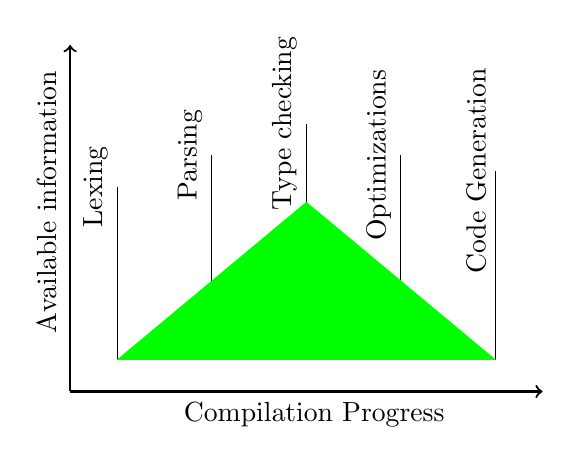
\begin{tikzpicture}[xscale=3, yscale=2]
\draw[->, thick] (-0.2,-0.2) -- (-0.2,2.0) node[xshift=-0.3cm, yshift=-0.2cm, left, rotate=90] {Available information};
\draw[->, thick] (-0.2,-0.2) -- (1.8,-0.2) node[xshift=-2.9cm, below] {Compilation Progress};
\draw (0.0,0) -- (0.0,1.1) node[above, rotate=90] {Lexing};
\draw (0.4,0) -- (0.4,1.3) node[above, rotate=90] {Parsing};
\draw (0.8,0) -- (0.8,1.5) node[above, rotate=90] {Type checking};
\draw (1.2,0) -- (1.2,1.3) node[above, rotate=90] {Optimizations};
\draw (1.6,0) -- (1.6,1.2) node[above, rotate=90] {Code Generation};
% horizontal line
\filldraw[color=green, fill=green] (0,0) -- (0.8,1.0) -- (1.6,0);
\end{tikzpicture}
  \caption{A visualization of the rough measurement of information present in each step of the compilation process. Type checking having the most information and lexing and code generation having the least amount of information.}
  \label{fig:InformationCompilation}
\end{center}
\end{figure}

Compilers have to construct a lot of complex information about the program. A visual some find helpful when reasoning about compilers is an imagined graph of ``available information``. Figure \ref{fig:InformationCompilation} tries to communicate the amount of information created in each step of compilation. The most important part being that we know a lot about the program in the type checking phase -- more than when doing syntactical analysis.

\subsection{Abstract Syntax Tree}
General purpose programming languages need to be recursive in their structure -- one might want a sub-expression inside another expression for example. Representing this structure inside a computer cannot simply be done with a simple list of values, the data-structures themselves must reflect the structure of the language. One very popular way of storing this recursive syntactical information is by using an abstract syntax tree (often referred to as an AST). An AST describes the structure of the program.


\begin{figure}[h!]
\centering
\begin{subfigure}{.5\textwidth}
  \begin{minted}[]{bnf}
<expr> ::= <num> | <expr> + <expr>

<num>  ::= 1 | 2 | 3
\end{minted}
\end{subfigure}
  \cprotect\caption{A simple grammar for integer expressions. Here an \verb|<expr>| is either a \verb|<num>|, so a simple number, or the it is a sum of 2 \verb|<expr>|.}
  \label{fig:bnfExpr}
\end{figure}
For example, consider the grammar for integer addition expressions described in grammar shown in Figure \ref{fig:bnfExpr}. The syntax understands whole numbers from 1 to 3 and the basic arithmetic operation addition (\verb!+!). Most notable is that the syntax is recursive and expressions can contain expressions in themselves. This BNF-like syntax is a bit simplified and the grammar is not necessarily in a good format. A better grammar would handle order of operations and avoid ambiguities -- which will be explained later.

The basic idea of the BNF is that we can expand each node -- and all expansions are valid ''programs'' in the language. Here valid means syntactically correct -- it does not mean the ideas expressed in the ''program'' are meaningful in any way. The rules expressed in the BNF say that an \verb|<expr>| might be replaced with either \verb|<num>| or \verb|<expr> + <expr>| And that a \verb|<num>| can be replaced with \verb|1| or \verb|2| or \verb|3|. All valid programs are \verb|<expr>| we can start expanding from there -- the simplest program might be \verb|1| since we can get this from expanding \verb|<expr> -> <num> -> 1|. But we could also do the expansions:
\begin{verbatim}
  <expr> -> <expr> + <expr>
         -> <expr> + <expr> + <expr>
         -> <expr> + <expr> + <num>
         -> <expr> + <expr> + 1
         -> <expr> + <num> + 1
         -> <expr> + 2 + 1
         -> <num> + 2 + 1
         -> 3 + 2 + 1
\end{verbatim}
These expansions can get quite repetitive so special notation is often used to abbreviate. This syntax is also so simple that the format expressed here is needlessly powerful. But the important detail here is that we do not know if we expand the left-most \verb|<expr>| or the right more \verb|<expr>| when we apply the rule \verb|<expr> ::= <expr> + <expr>|. To learn more we recommend any book on automatas or parsers. 

We can write a simple ''program'' that is a part of the language described by Figure \ref{fig:bnfExpr}. Some small valid ''programs'' are: \verb!1!, and \verb!1 + 1!. But we will focus on the expression \verb!1 + 2 + 3! -- which has two additions.

Looking at the expression \verb!1 + 2 + 3! it is obvious that the expressions should evaluate to 6. What is not obvious is how a computer should evaluate this expression. We can namely construct two different abstract syntax trees (and two different parse trees) for the program \verb!1 + 2 + 3!. When parsing the program to a syntax tree we have to make the conscious decisions of what node is placed on top.


\begin{figure}[h!]
\centering
\begin{subfigure}{.5\textwidth}
\centering
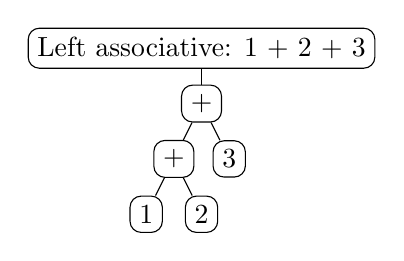
\begin{tikzpicture}[
  sibling distance=2em,
  level distance=2em,
  every node/.style = {shape=rectangle, rounded corners, draw, align=center}
]
  \node {Left associative: 1 + 2 + 3}
          child {node {+}
            child {node {+}
              child {node {1}}
              child {node {2}}
            }
            child {node {3}}
          };
\end{tikzpicture}
\end{subfigure}%
\begin{subfigure}{.5\textwidth}
\centering
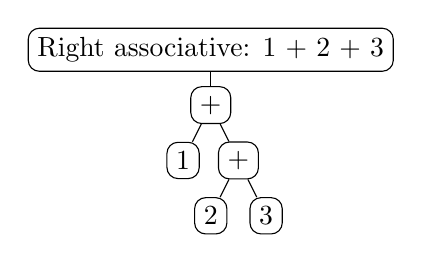
\begin{tikzpicture}[
  sibling distance=2em,
  level distance=2em,
  every node/.style = {shape=rectangle, rounded corners, draw, align=center}
]
  \node {Right associative: 1 + 2 + 3}
          child {node {+}
            child {node {1}}
            child {node {+}
              child {node {2}}
              child {node {3}}
            }
          };
\end{tikzpicture}
\end{subfigure}
  \caption{Two example syntax tree -- illustrating ambiguity in the grammar and the difference between left and right associativity.}
  \label{fig:astExpr}
\end{figure}

Figure \ref{fig:astExpr} shows the two different associativities that causes \verb!1 + 2 + 3! to be interpreted as either \verb!(1 + (2 + 3))! or \verb!((1 + 2) + 3)!. There is not much difference between these mathematical expressions -- they are even considered equivalent since addition is associative for integers. The associativity property is unfortunately very rare in the real world of effectful-programming. If evaluating an expression in this language had side-effects -- for example printing the result, different associativities would cause different outputs. One of the programs would print \verb+1 2 3 3 6+ while the other would print \verb+1 2 3 5 6+ (ofcourse dependent on how the expressions are evaluated). This is what is called an ambiguity -- and an abstract syntax tree makes it clear how the compiler internally understands this addition.

Making additions have side-effects is not the only way to get non-associative additions, one could use a less well-behaved addition like that found in the IEEE floating point standard -- since any form of rounding is non-associative. Unfortunately infinite precision is quite rare when storage is finite.

There are different operations which can be done to an abstract syntax tree. In our very simple example of integer additions it would make sense to fold the constants and replace the entire AST with the constant 6 -- but to do that we would have to know the associativity of the \verb!+!-operator.

Because of its flexibility the AST is very a very popular format to output from the parsing stage. In the Spade-compiler the AST is annotated with type information as it is discovered -- this annotated AST is then either to a language server or a code generation phase.

\section{Syntax and Semantics}
There are two concepts when talking about language, syntax and semantics. Syntax is the structure of the language, how the words are placed next to each other and what makes a valid sentence. Programming languages also have a notion of sentences and validity, and the word for syntax applies there as well. Syntax can also be used to describe natural languages.

Writing words down with valid syntax is all well and good, but they also need to be meaningful. The meaning of a sentence is called the semantics. This holds for programming languages as well. The expression \verb+a * b+ is syntactically valid, but lacks any kind of semantic without a definition for what '*' means and what \verb+a+ and \verb+b+ actually are, the example of \verb+a * b+ could be a multiplication between two terms but it could also be a declaration of a pointer variable in C.

Syntax and semantics are related, and the syntax can affect the semantics. The important distinction is that semantics is the meaning and syntax is the structure of the text.

\section{Type Checking} % Maybe `inner layers`?
\label{sec:TypeChecking}
Type checking is a way of making sure the program is internally consistent -- there are no contradictions inside to program to the program itself. Type checking can be done in different ways with different pros, cons or preferences \cite{src:TypeCheckersBook}. The type checker in Spade can infer types and deduce things about the program, like ``the first argument is a 3-bit integer value, but you gave an enum`` \cite{src:spadeAnHDL}.

For details regarding the Spade type checker, see Section \ref{sec:TheSpadeTypechecker} which discusses implementation details.

The type checker in Spade is a Damas-Hindley-Milner type checker \cite{src:DamasHindleyMilner}. This means it stops on the first error and can deduce types to their most general form. So if asked to type check the identity function (a function that takes one value and returns the value as is, the function does nothing) the type checker would be able to deduce that the argument could have any type, but that the type is the same as the type of the returned value, with only the body of the function.\cite{src:DamasHindleyMilner}

There is also a connected topic of type inference -- a program that guesses the types of expressions based on the context. A sufficiently good typeinferer could be used to check the types of the program and can easily be made into a type checker. It is infact upon this idea that the Damas-Hindley-Milner typechecker works. In this work, we consider typechecking and typeinference the same operations -- since Spade implements typechecking using typeinference. This equivalence is not the same for all typecheckers, since some only check types without inferring.

\subsection{Unification}
\label{sec:Unification}
A Damas-Hindley-Milner type checker is a very simple typechecker and is based upon one simple idea: typeinference is a constraint satisfaction problem with \textit{only} equivalence-constraints. The idea of the typechecking and typeinference is to simply find types that have to be equal for the program to function. Most of these small rules are painfully simple -- like: ''adding two numbers gives you a number'', or ''calling a function results in a type with the return value of the called function''. What really drives these simple rules is a process called unification. Unification is a way to propagate these equality constraints. This is proven to be correct, given that all expressions without sub-expressions have a type.

This unification property is also found in logic-programming, which is not a coincidence but rather an effect of the Curry–Howard isomorphism. \cite{src:curryHowardIso}

We find examples useful to quickly get basic understanding of a topic, so we will outline the type checking of a simple program and how the unification step would work. We will typecheck the simple program in Figure \ref{fig:progUni}.

\begin{figure}[h!]
\centering
\begin{subfigure}{.5\textwidth}
  \begin{minted}[linenos]{rust}
fn add<A> : (A, A) -> A

fn main { add(add(1, 2), "abc") }
\end{minted}
  \end{subfigure}
  \caption{A simple dummy program to show unification. A simple ''add'' function is defined which takes 2 arguments of the same type and returns that type. Types are denoted with uppercase letters and language constructs are defined using lowercase letters.}
  \label{fig:progUni}
\end{figure}

\begin{figure}[h!]
\centering
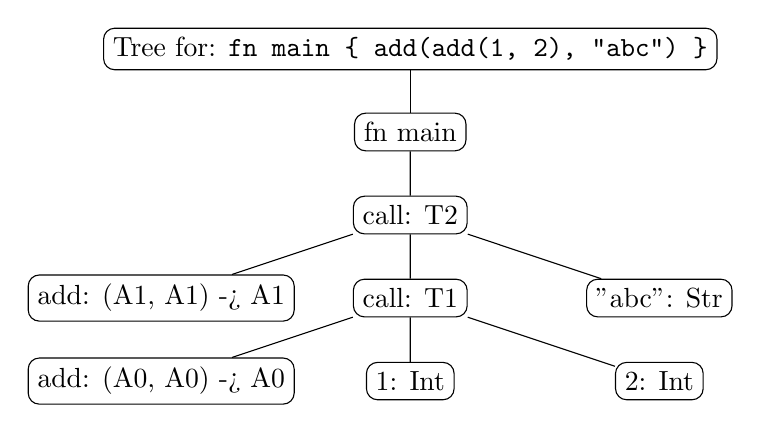
\begin{tikzpicture}[
  sibling distance=9em,
  level distance=3em,
  every node/.style = {shape=rectangle, rounded corners, draw, align=center}
]
  \node {Tree for: \verb|fn main { add(add(1, 2), "abc") }|}
          child {node {fn main}
              child {node {call: T2}
                    child {node {add: (A1, A1) -> A1}}
                    child {node {call: T1}
                        child {node {add: (A0, A0) -> A0}}
                        child {node {1: Int}}
                        child {node {2: Int}}
                    }
                    child {node {"abc": Str}}
              }
          };
\end{tikzpicture}
  \cprotect\caption{The syntax tree for \verb|fn main { add(add(1, 2), "abc") }| with the generated type variables before we have annotated all the types.}
  \label{fig:progUniTree}
\end{figure}

\begin{figure}[h!]
\centering
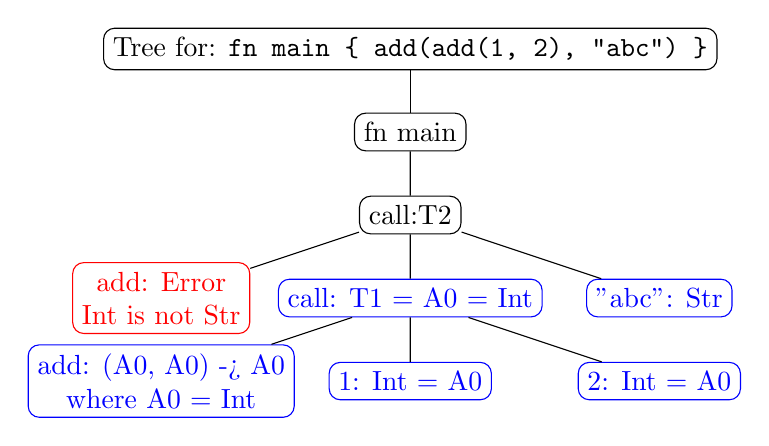
\begin{tikzpicture}[
  sibling distance=9em,
  level distance=3em,
  every node/.style = {shape=rectangle, rounded corners, draw, align=center}
]
  \node {Tree for: \verb|fn main { add(add(1, 2), "abc") }|}
          child {node {fn main}
              child {node {call:T2}
                    child {node[color=red] {add: Error\\Int is not Str}}
                    child {node[color=blue] {call: T1 = A0 = Int}
                        child {node[color=blue] {add: (A0, A0) -> A0\\where A0 = Int}}
                        child {node[color=blue] {1: Int = A0}}
                        child {node[color=blue] {2: Int = A0}}
                    }
                    child {node[color=blue] {"abc": Str}}
              }
          };
\end{tikzpicture}
  \cprotect\caption{The syntax tree for \verb|fn main { add(add(1, 2), "abc") }| with the generated type variables after we have inferred as far as we can. We see an error marked in red and finished nodes which are marked in blue. The error was found when we tried to unify \verb|Str| with \verb|Int| since the call requires both arguments to be the same type.}
  \label{fig:progUniTreeAfter}
\end{figure}


Let us assume that we have two types in our language \verb+Int+ and \verb+Str+. We start by giving each construct a unique type variable. (The unique type variable is mainly to aid explanation. There are more resource efficient ways of implementing Damas-Hindley-Milner.) We then evaluate the syntax tree bottom up -- the syntax tree is shown in Figure \ref{fig:progUniTree}. We will also assume the rules: 
\begin{enumerate}
  \item Integer-constants have the type \verb+Int+.
  \item String-constants have the type \verb+Str+.
  \item Calling a function means the types of the arguments can be unified with the parameters and the whole expression evaluates to the return type of the function. Evaluating rule (3) always gives a new type ''A'', we will keep track of these with numbered suffixes.
\end{enumerate}
These 3 simple rules let us type check and typeinfer the expression in the main-function.

In this explanation the \verb+:+ operator denotes that an expression on the left has a known type on the right, so \verb+1:Int+ means the expressions \verb+1+ has type \verb+Int+. We will also denote the unifications of types, so \verb+A9=A8+ means the type \verb+A9+ is the same types as \verb+A8+. We first of all know the type of all the simple expressions -- thanks to rules (1) and (2) -- that means \verb+1:Int+, \verb+2:Int+ and \verb+"abc":Str+. We can now solve \verb+add(1, 2)+ by applying rule (3) to \verb+add:(A0, A0) -> A0+ and \verb+add(1, 2):T1+, we can unify \verb+(Int, Int)+ and \verb+(A0, A0)+, which gives \verb+A0=Int+. We also get \verb+T1=A0=Int+ which gives us \verb+add(1, 2):Int+. The more complex expression is now inferable \verb+add(add(1, 2), "abc"):T2+, we unify \verb+(T1, Str)+ and \verb+(A1, A1)+ which gives us a contradiction, since \verb+T1=Int=/=Str+ -- this would result in a type error which might be thrown by the compiler. This result is shown in the Figure \ref{fig:progUniTreeAfter}

In conclusion, unification lets us define two types as the same type and send all this information as far as we want in a program -- there are programming languages with global type-inference for example. But the method described by Damas-Hindley-Milner is limited to equality-constraints which has some limitations in what types can be expressed.

\subsection{Monomorphisation}
\label{sec:Monomorphisation}
After all the type checking and typeinference has been done monmorphisation can take place. This phase turns generic functions into concrete function -- that is to say all functions with generics like \verb+fn add<A>(x: A, y: A) -> A+ are given concrete types like \verb+fn add(x: i32, y: i32) -> i32+. This means the same code can lead to multiple function bodies. Monomorphisation creates a new instance of a function for each of the generic arguments given, and Rust does something similar. \cite{src:rustMono}

Monomorphisation is often considered a performance optimization, but for HDLs this step is absolutely required since the hardware does not handle function pointers or any kind of indirect control flow. So modeling virtual methods from object oriented programming could be quite tricky, this means the resource usage would grow with the number of implementations for a virtual method, since we cannot know at compile time which of these results is the right one (unless we use monomorphisation) -- the scaling of this solution negates all the benefits of virtual methods and is not a good fit for FPGA development where resources are scarce. 

\subsection{The Lambda Cube}
% NOTE[et]: I'm not sure how I feel about this section, I feel like this kind of information is too abstract to help people understand this work...
\label{sec:lambdaCube}
Typesystems are complex, and there are alot of them. But typesystems are also a very theoretical study, and comes from the idea of type theory. Type theory is a branch of mathematics that focuses on and reaching conclusions using types. A good place to start to understand at least parts of the field is to look at lambda calculus -- a kind of ''proramming language'' similar to a turing machine in that it is a mathematical construct for computation. Lambda calculus allows function definitions and from that natural numbers and boolean operations are constructed -- this is quite a deep field and is not the exact topic of this work, so details will be left a bit hazy. But the lambda calculus is a very good playground for typesystems, since all computable computations can be reduced to an expression in lambda calculus and lambda calculas has functions and function calls as its only constructs.

\begin{figure}[h!]
\begin{center}
\begin{tikzpicture}
  % Nodes
  % Simply typed
  \node[minimum width=1cm, minimum height=1cm] (st) at (0,0) {$\lambda{}\hspace{-0.3em}\rightarrow$};

  % System F
  \node[minimum width=1cm, minimum height=1cm] (sf) at (0,4) {$\lambda$2};
  \node[minimum width=1cm, minimum height=1cm] (lp) at (4,0) {$\lambda$P};
  \node[minimum width=1cm, minimum height=1cm] (fw) at (2,2) {$\lambda\underline{\omega}$};

  \node[minimum width=1cm, minimum height=1cm] (fW) at (2,6) {$\lambda\omega$};
  \node[minimum width=1cm, minimum height=1cm] (lpo) at (6,2) {$\lambda{}P\underline{\omega}$};
  \node[minimum width=1cm, minimum height=1cm] (lp2) at (4,4) {$\lambda$P2};

  % Calculus of Construction
  \node[minimum width=1cm, minimum height=1cm] (cc) at (6,6) {$\lambda$C};
  
  % Arrows
  \draw[->] (st) -- (sf);
  \draw[->] (st) -- (lp);
  \draw[->] (st) -- (fw);

  \draw[->] (fw) -- (fW);
  \draw[->] (fw) -- (lpo);

  \draw[->] (lp) -- (lp2);
  \draw[->] (lp) -- (lpo);

  \draw[->] (sf) -- (fW);
  \draw[->] (sf) -- (lp2);

  \draw[->] (lp2) -- (cc);
  \draw[->] (lpo) -- (cc);
  \draw[->] (fW) -- (cc);

\end{tikzpicture}
  \caption{The lambda cube}
  \label{fig:lambdaCube}
\end{center}
\end{figure}

When talking about typesystems for the lambda calculus you always limit the power of the language, but you can get some other niceities like bounded execution times. The lambda cube (as shown in Figure \ref{fig:lambdaCube}) is a way to categorize these different type systems in order of power. Each dimension of the cube is a different kind of feature for a typesystem. The bottom left of the lambda cube is the simply typed lambda calculus, where only terms working on terms is allows (this is usually called functions). The arrows going in the $\rightarrow$-direction (not the same arrow as in $\lambda{}\hspace{-0.3em}\rightarrow$) mean there are types that can affect terms, known as dependent types and is considered by some quite esoteric but is mostly used in computer proof systems like Coq or Agda -- these languages express mathematical truths not necessarily usable programs though the feature allows for more computation power. The arrows in the $\nearrow$-direction signals types that act on other types, this is mostly considered a convince and does not increase the power but can increase the expressiveness one for example higher-kinded types in Haskell or PureScript. Finally there's arrows in the $\uparrow$-direction which means terms that can affect types -- or polymorphism as it is known in C++ or Java. In a sense the lambda cube can be thought of as a map for typesystems and their complexities. The most powerful of these typesystems is the calculus of construction, and it has all these 3 typesystem features and it also has the most computational power of them all, meaning all of the other typesystems can be constructed by removing features for the calculus of construction.

Most typesystems for programming languages can be mapped to one of these theoretical type systems. Spade can be mapped to somewhere around $\lambda\omega$ since it has polymorphic functions and types that work on other types in the form of \verb+ConstraintExpr+ -- though it is not as general as something like the Haskell typesystem so one could argue that Spade has partial higher kinded types, which puts it between $\lambda\omega$ and $\lambda{}2$. Languages like Coq have all the bells and whistles of calculus of construction and is thus considered more complex. There is also things like Elm which falls somewhere between $\lambda{}2$ and $\lambda\omega$. This means Spade has a typesystem that is about as complex and powerful as that of Elm. So constructs that can be expressed in Elm should also be expressible in the Spade typesystem, this is a good sanity check for language features that one wishes to add. Wordlength inference could be mapped to a record where each field is an integer and the field is present if the integer falls in the available range, the functions for these computations could not be expressed inside the Elm language since it is deliberately locked down, but if one had access the compiler one could unlock the full power and easily write these functions, this should give some theoretical basis for the possibility of this work.

\section{Spade}
Spade is a HDL that takes a lot of inspiration from Rust to create a more modern HDL (Hardware Description Language). Spade has syntax which mimics that of Rust and tries to remove problems people have when using other HDLs like System Verilog. One of the biggest features of Spade is the static type checking which allows programs to be verified before even being synthesized -- creating a faster iteration loop.
\cite{src:spadeSomething} \cite{src:spadeAnHDL}

\subsection{Swim}
The Spade-ecosystem has a build-tool call Swim. Swim orchestrates things like running PNR, running synthesis tools, installing dependencies, generating basic projects and compiling Spade-code. Swim is the best way to handle any Spade project.

\subsection{Spade syntax}
All programming languages have some kind of syntax -- and Spade has taken a lot of inspiration from Rust in this domain but make additions and tweaks due to the different domain of the language. This section contains a short version of the relevant Spade syntax, there is more to the Spade-language but some short snippets are explained here.

Spade has multiple novel constructs there are: entities which can hold state while doing operations (think stateful functions to get an overview), pipelines that allow computations to stretch over multiple cycles and functions which are very much like functions in your favorite programming language. This guide will focus mostly on functions as a language construct since they are very well documented and most people who have written code has used something similar.

\begin{figure}[h!]
\begin{minted}[linenos]{rust}
fn identity(x: int<5>) -> int<5> {
  x
}
\end{minted}
  \caption{The definition of a function which does nothing with its argument.}
  \label{fig:SpadeExample1}
\end{figure}

The code in Figure \ref{fig:SpadeExample1} show a simple definition of a function which directly returns the argument passed to it. The function is defined by the \verb+fn+-keyword similar to Rust. Just like Rust the type of the argument comes after its name, to the joy of the type theorists. The \verb+int+ type -- which means integer and is the main focus of this work -- takes a type argument that is passed inside of the angle-brackets (\verb+<>+). The argument passed to the \verb+int+-type is its wordlength, how many bits the integer fills up. A stark contrast to languages like C where you usually only have options that are powers of two. If the last statement in a function is an expression, it is automatically returned, again borrowed from Rust.

\begin{figure}[h!]
\begin{minted}[linenos]{rust}
fn calculate(x: int<5>) -> int<7> {
  let partial_result: int<3> = some_function(3);
  x + 1 * 2 - partial_result
}
\end{minted}
  \caption{Some mathematical operations that }
  \label{fig:SpadeExampleOps}
\end{figure}

Simple operations like multiplication, subtraction and addition exist and are expressed as one would expect as shown in Figure \ref{fig:SpadeExampleOps}. Functions and entities can be called with parenthesis and any Rust-user should feel right at home. Statements are separated by semicolons.

\begin{figure}[h!]
\begin{minted}[linenos]{rust}
fn generics<#A, #B, T>(x: int<A>, t: T) -> int<B> {
  if t == t {
    x + x
  } else {
    0
  }
}
\end{minted}
  \caption{An if-expression and some generic arguments passed to a function.}
  \label{fig:SpadeExample2}
\end{figure}

Spade has generics, which are bound to functions the function \verb+generics+ that is defined in Figure \ref{fig:SpadeExample2}. There are two different kinds of generics, those that have a \verb+#+-sign before them and those that do not. The \verb+#+ indicate a compile time integer, and are used to aid the compiler with inferring the wordlength of expressions between functions. The remaining generics are type variables which are types passed to types. There are also if-expressions in the language that allow branching, these use the same implicit returns as the function bodies.

There are more language constructs in Spade, but these constructs are deemed irrelevant for this work -- for a more through reference see the Spade-book\footnote{\url{https://docs.spade-lang.org/}}.

\subsection{The Spade Type checker}
\label{sec:TheSpadeType checker}
Since Spade is a statically typed language the compiler has a type checker. The Spade typechecker is a variant of Damas-Hindley-Milner and the intricacies of this class of type system is discussed in Section \ref{sec:TypeChecking} which discusses typechecking more broadly while this section mentions the specifics of the implementation in the Spade compiler before any changes were made.

The Spade type checker walks through he syntax tree of the program applying rules to each node, unifying (Section \ref{sec:Unification}) types which have to be equal for the program to be valid. Each expression in Spade has a corresponding typevariable which holds the type of the expression. These typevariables can also contain type variables inside them, so types with generics are encoded with their generic arguments. The implementation looks a bit like: \verb+TypeVar(Id, Vec<TypeVar>)+, this is a bit simplified but the details are enough to understand the rest of this work. The unification of the outer type variable would also cause the inner type variables to be unified.

Besides type variables there are constraints and requirements -- they do different things so the synonyms make them a bit confusing to talk about. \verb+Requirement+ is the least relevant, and handles methods and fields that are ''required'' to exist on types, but also that a certain typevariable has to hold an integer of a certain value. After a \verb+Requirement+ is satisfied the affected type variables are updated and the \verb+Requirement+ is discarded.

There are also \verb+ConstraintExpr+, which are used and referenced a lot more in this work. \verb+ConstraintExpr+ handle compile time integers and have functionality for adding (\verb+Sum+), subtracting (\verb+Sub+), variables (\verb+Var+), constants (\verb+Integer+) and evaluating using $\text{floor}(\log_2{n} + 1)$ where $n$ is the compiletime integer (\verb+BitsToRepresent+) -- the logarithm operation is used to find the number of bits a value needs to be represented. These constraints are solved in a similar way to the constraints, are removed when they are satisfied and relevant typevariables are then updated. The \verb+ConstraintExpr+ lack syntax in the spade language and cannot be expressed outside of the type checker.

\subsection{Wordlength Inference in Spade}
\label{sec:TheProblem}
Most values in Spade take up bits or space in the run time environment. Wordlength inference is mostly concerned with integers -- so consider positive numbers without a decimal. Consider a program with a counter that resets to 0 after counting to 3, we do not need 32 bits to represent it. The cost of storing a number with 32 bits compared to 2 bits could be large if it requires a larger FPGA, extra circuit components or a different power rating. Compared to software engineering of programs for general purpose computers where memory is considered abundant, FPGAs are limited in memory and computations use parts of the FPGA which causes HDLs to be designed differently to a general purpose programming languages.

Wordlength inference is the compiler understanding what wordlength -- the number of bits -- is needed to store a value. Inferring this value well results in  good resource usage and requires less manual intervention. Doing it poorly or not at all either requires users to manually specify the wordlength of each value, or hardware that is inefficient.

In Spade integer types are written using the \verb|int| keyword, and wordlength is specified by passing a generic to the integer type. \verb|int<3>| specifies an integer that spans 3 bits and holds values between $-(2^2) = -4$ and $2^2 - 1 = 3$. Spade also infers wordlengths based on the number of additons and multiplications -- so one addition adds one extra bit of required precision while a multiplication adds the wordlengths together. This approach means that equivalent expressions require different wordlengths depending on the number of additions and multiplications used to express it. 

\begin{figure}[h!]
\centering
\begin{minted}[linenos]{rust}
fn f(a: int<3>) -> int<4> {
  a + 1 + 1
}

entity main(clk: clock, rst: bool) -> int<4> {
  f(3)
}
\end{minted}
\caption{A simple spade program that does not compile, showing the current limitations of wordlength inference.}
\label{figSimpleFaultSpade}
\end{figure}

\begin{figure}[h!]
\centering
  \begin{minted}[]{text}
error: Type error
  |- src/simple\_fault.spade:1:27
  |
1 |   fn f(a: int<3>) -> int<4> {
  |                      ------ int<4> type specified here
  | |---------------------------^
2 | |   a + 1 + 1
3 | | }
  | |-^ Found type int<5>
  |
  = Expected: 4
  =       in: int<4>
  =      Got: 5
  =       in: int<5>

Error: aborting due to previous error
\end{minted}
\caption{The output from the compiler when trying to compile the program in Figure \ref{figSimpleFaultSpade}}
\label{figSimpleFaultSpadeCompileOutput}
\end{figure}

Consider the program in Figure \ref{figSimpleFaultSpade}. The function \textit{f} adds 3 values together, two of which are known constants. We also know that $2^2 + 2 < 2^3$ -- we should be able to fit the result of the addition into the 4 bit word without loss of data. The compiler does not agree as seen in the compiler output in Figure \ref{figSimpleFaultSpadeCompileOutput} where it claims we need 5 bits to store this value. This problem might seem inconsequential since calculating constant expressions during compilation would fix this, as seen by the program in Figure \ref{figSimpleCorrectSpade} compiling without worries. Adding constants is only the tip of the iceberg that is this problem. The problem here is much deeper, and is a direct cause of the implementation of type checking and wordlength inference directly.

\begin{figure}[h!]
\centering
  \begin{minted}[linenos]{rust}
fn f(a: int<3>) -> int<4> {
  a + 2
}

entity main(clk: clock, rst: bool) -> int<4> {
  f(3)
}
\end{minted}
  \caption{``simple\_correct.spade`` A spade program that does compile and is equivalent to the program in Figure \ref{figSimpleFaultSpade}}
\label{figSimpleCorrectSpade}
\end{figure}

The Spade compiler implements a Damas-Hindley–Milner type checker -- discussed in more detail in Section \ref{sec:TypeChecking}. Damas-Hindley-Milner runs in almost linear time (if implemented correctly) but is not complete. The completeness property for type checkers means there are programs which are correct but that the type checker will not recognize as correct. The programs from Figures \ref{figSimpleFaultSpade} and \ref{figSimpleCorrectSpade} are an example of this. This observation is important since it means this is not a bug, but a limitation of the typechecking algorithm itself.

\begin{figure}[h!]
\centering
  \begin{minted}[linenos]{rust}
fn f(a: int<3>) -> int<4> {
  trunc(a + 1 + 1)
}

entity main(clk: clock, rst: bool) -> int<4> {
  f(3)
}
\end{minted}
  \caption{``trunc\_correct.spade`` A spade program that does compile and is equivalent to the program in Figure \ref{figSimpleFaultSpade}, but here we used a truncation operation to remove bits from the integer.}
\label{figSimpleTruncSpade}
\end{figure}

There is also another way the Spade program can be changed to make it compile. Figure \ref{figSimpleTruncSpade} adds a trunction operation to the expression in \verb+f+. The truncation operation, called \verb+trunc+, shortens the wordlength of an integer. This shortening sometimes causes information to be discarded -- but not always. The code in Figure \ref{figSimpleTruncSpade} shows a ''safe'' truncation, since no information will be discarded in this case. The \verb+trunc+-operation can be used erroneously and cause faults which might be hard to find.

\begin{figure}[h!]
\centering
\begin{verbatim}
trunc<4, 3>(sb1010) = sb010 = 2
sext<4, 5>(sb1010) = sb11010 = -5
zext<4, 5>(sb1010) = sb01010 = 10
\end{verbatim}
  \caption{3 Short examples for operations in spade which affect the wordlength. All the numbers are encoded using twos compliment without anyhidden bits, the wordlength is the number of 0s and 1s in the bit-string.}
\label{figSext}
\end{figure}

In addition to \verb+trunc+ there is also \verb+sext+ and \verb+zext+ which increase wordlengths. \verb+sext+ is a ''sign extension'' and increases the wordlength of the integer while keeping the sign byte the same. \verb+zext+ is a zero extension and pads the integer with zeroes to increase the wordlength. Some simple examples are available in Figure \ref{figSext} which shows 3 examples on the binary integer \verb+sb1010+ -- encoded here using twos-compliment and we assume no hidden bits --  which is -5 in decimal. Each of the operations take type-parameter, the Spade compiler usually infers these, the first type parameter denotes the ingoing wordlength and the second the outgoing wordlength. Of special interest is the sign extension, since it does not change the numerical value of this negative integer, the padding of the bit-string is done with the leftmost-bit (the ''sign''-bit) to keep the numerical value. The ''zero extension'' naively inserts zeroes -- which correctly keeps the values for positive numbers but here results in a wild 10 appearing. The truncation simply chops of the leftmost bits and calls it a day, if there was information there the information would be lost.

\subsection{HIR-lowering}
\begin{figure}[h!]
  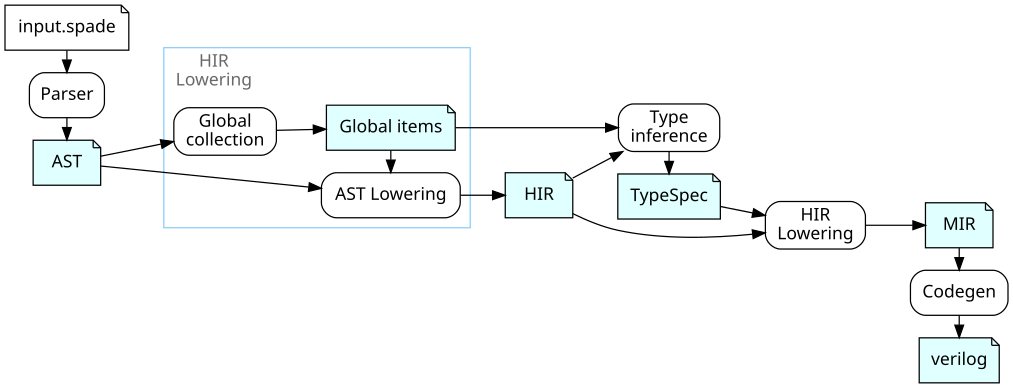
\includegraphics[width=\textwidth]{architecture.png}
  \caption{An over view of the spade compiler, taken from the Spade architecture documentation\cite{src:Architecture}.}
  \label{figArch}
\end{figure}

Figure \ref{figArch} show the overarching architecture of the Spade language. Since the level of abstraction between Spade and Spades compile target is so different. Translating between these abstraction levels is quite complex, and is done in steps. The relevant step in this chain is called \verb+HIR-lowering+, HIR stands for ''Higher Intermediate Representation'' and is the first of these steps, the later steps are not as relevant to the type checking but are very interesting when compiling. The HIR has been typechecked and monomorphised (Section \ref{sec:Monomorphisation})\cite{src:Architecture}.

\subsection{Rust}
Rust is a statically typed general purpose systems programming language. The language has recently seen a lot of popularity and boasts features like high performance, reliable software and increased developer productivity. It is also the language that is used to write the Spade compiler. \cite{src:Rust}

\subsubsection{BigInt}
Since Spade can express large wordlengths the maximum values cannot always be expressed in smaller sized integers. A solution to this is to use what is called ''BigInt'', it is an integer which has arbitrary precision. This means that really large numbers can be represented. This representation is very slow compared to ''normal'' integers and the size of these BigInts can grow unbounded.

\subsubsection{BigRational}
Besides BigInt one can define a real number with arbitrary precision, this is trivial if you have a BigInt since all rational numbers can be expressed as a ratio between two integers. This representation is also very slow compared to ''normal'' floats and the size of these BigRationals can grow unbounded. 


\section{Interval Arithmetic, Affine Arithmetic and Self Validating Numerical Methods}
\label{sec:IAndAA}

Affine arithmetic and interval arithmetic are two common ways to estimate the value of arbitrary mathematical expressions. AA and IA can be applied to estimate bounds for mathematical functions and thus all things that can be modeled by mathematical functions. Since programs can be modeled using mathematical expressions IA and AA have a place in static analysis of programs, which is the focuses of this work. These methods are often referred to as over-estimation or self validating numerical methods.

\subsection{Interval Arithmetic}
Interval arithmetic operates on intervals, as the name implies. A value -- or in the context of a program, a variable -- has a smallest and largest value it can assume. Consider \verb`x = random_real()`, where \verb`random_real` generates a random value in the range $[0, 1]$. We can express this in interval arithmetic as $\bar{x} = [0, 1]$, intervals will be denoted with a bar on top to separate them from the variables. Note especially that the true value of $x$ lies in the interval $\bar{x}$. In this example we know $0 \leq x \leq 1$, also written as $x \in [0, 1]$. These intervals can be added, negated, and so on, to give you an estimate of an arbitrary expression. The empty interval is also defined and written as $[]$. The empty interval usually denotes expressions or code that cannot be reached or evaluated -- it a very sane default value for merging together multiple branchen in a Spade match-statement, since if there are no matches we would infact have unreachable code.

\subsubsection{Interval Arithmetic: An Example and Limitations}
Some of the rules for interval arithmetic are:
\begin{enumerate}
  \item $n * [a, b] = [n * a, n * b]$
  \item $[a, b] - [c, d] = [a - d, b - c])$
  \item $[a, b] + [c, d] = [a + c, b + d]$
\end{enumerate}

We will be using the expression $2x + z - z$ as an example where $x = [0, 1], z = [1, 3]$. This mean we have the expression after expanding the variables which we can calculate:
\begin{align*}
  2x + z - z \\
  =^{\text{expansion}} \quad & 2 * [0, 1] + [1, 3] - [1, 3] \\
  =^{1}                \quad & [2 * 0, 2 * 1] + [1, 3] - [1, 3] \\
  =^{2}                \quad & [0, 2] + [1 - 3, 3 - 1] \\
  =^{\text{simplify}}  \quad & [0, 2] + [-2, 2] \\
  =^{3}                \quad & [0 + -2, 2 + 4] \\
  =^{\text{simplify}}  \quad & [2, 4]
\end{align*}
We start by applying the scaling rule (1) -- then the subtraction rule (2) and last the addition rule (3) giving us $2x + z - z = [-2, 4]$. This means the expression $2x + z - z$ with the context $x = [0, 1], z = [1, 3]$ always lies in the range $[-2, 4]$.
\label{sec:prevResultIA}

The conclusion we've reached is true, but the estimate is larger than it necessarily needs to be. Notice that subtracting the value $z$ from itself should result in $0$, which is a perfectly valid point and correct point. This is a limitation of the interval arithmetic. Interval arithmetic does not reason about the expressions that came before it and how they combine, and this limitation would exist if used to do static analysis of programs. 

\subsection{Affine Arithmetic}
Affine arithmetic (AA) works similarly to interval arithmetic (IA), but has a memory of where values come from and can reason about their combinations at a higher level. But AA understand the relations between variables we evaluate if we provide the context. AA can more accurately calculate expressions like $a - a$ since it understands that $a$ and $a$ must hold the same value. That said, AA does not produce strictly better results than IA in all circumstances.\cite{src:affAri}

Though affine arithmetic is more sophisticated it does not always produce better results, interval arithmetic can for some computations produce tighter bounds. There are other methods for overestimation that are considered more sophisticated like ME-gPC \cite{src:MEgPC} and modified affine arithmetic, but the extra complexity can be added later if it is found to be needed. ME-gPC was not considered for this work due to its complexity -- but it is a good extension to the techniques explained in this work. Affine arithmetic and interval arithmetic are the simplest methods that offer enough complexity to make this work interesting.

\subsubsection{Affine Arithmetic: An Example and Limitations}
In affine arithmetic there is a concept of noise symbols ($e_i$ where $i$ is a real number between $[-1, 1]$) and the numbers half width ($x_i$ where $i$ is a real number). A linear combination of these noise symbols is a reasonable way to represent a "number" when reasoning about affine arithmetic, $\hat{x} = x_0 + x_1e_1 + x_2e_2 + \dots$. These terms can then be combined using similar rules to interval arithmetic. Of special interest is the first term, and the lack of a noise variable ($e_0$ is what one would have expected) -- the first term can be thought of as shifting the uncertainty up and down number line. Furthermore, we can consider the expression $\hat{x} - \hat{x}$, and since we have noise variables we get the expected result of $0$.\cite{src:affAri} 

Here is an excerpt of relevant rules for affine arithmetic.
\begin{enumerate}
  \item $[a, b] \Rightarrow x_0 = (a + b) / 2, x_n = (a - b) / 2$ where $n$ is unique, this maps a range to its affine form $\hat{x}$
  \item $n * \hat{x} = \hat{z}$ where $z_n = n * x_n$
  \item $-\hat{x} = \hat{z}$ where $z_n = -x_n$
  \item $\hat{x} + \hat{y} = \hat{z}$ where $z_n = x_n + y_n$
  \item $\hat{x} \Rightarrow [a, b]$ where $a = x_0 + \sum_{1\dots{}n}{x_ie_i}: e_n = -1$ and $b = x_0 + \sum_{1\dots{}n}{x_ie_i}: e_n = 1$
\end{enumerate}

Time for a simple example! Let us use $2x + z - z$ where $x = [0, 1], z = [1, 3]$.
We start by expanding the context $x = [0, 1], z = [1, 3]$ from ranges to their affine form using (rule 1), $\hat{x} = 0.5 + 0.5e_x, \hat{z} = 2 + 1e_z$, we can then expand the expression and use our other rules.

\begin{align*}
    2x + z - z \\
    =^{\text{expansion}} \quad & 2 * (0.5 + 0.5e_x) + (2 + e_z) - (2 + e_z) \\
    =^{2} \quad & (1 + e_x) + (2 + e_z) - (2 + e_z) \\
    =^{3} \quad & (1 + e_x) + (2 + e_z) + (-2 + -e_z) \\
    =^{4} \quad & (3 + e_x + e_z) + (-2 + -e_z) \\
    =^{4} \quad & (1 + e_x + 0e_z) \\
    \Rightarrow^{5} \quad & [1 - 1 - 0, 1 + 1 + 0] = [0, 2]\\
\end{align*}

We start by applying the scaling rule (2), then we simplify subtraction to a negation and an addition using rule (3). Now we just have a final summation using rule (4) twice. After all this the expression can be changed to a range using rule (5) which gives us $[0, 2]$, which is exactly $2x$ -- the answer that would have been preferred in Section \ref{sec:prevResultIA}. There is of course nothing magical going on here, all of these calculations are just simple algebra and we could just as easily have expanded the first expressions directly without using any special rules. However, this simplification cannot always be used. 

\subsection{When Interval Arithmetic Is Better Than Affine Arithmetic}
Affine arithmetic may seem like the superior option in all cases -- this is not true. Affine arithmetic has trouble with multiplication, and has to add extra noise in order to constantly overestimate. If we consider the simple case of multiplying two expressions in affine form $a + e_a$ and $b + e_b$ where $e_a$ and $e_b$ are noise variables we can use simple multiplication rules we get $(a + e_a)(b + e_b) = ab + ae_b + be_a + e_ae_b$, this is almost a valid affine form expression. But the pesky $e_ae_b$ term is illegal in AA. Since we have not defined what multiplying noise variables is (this is infact the next improvement we can do and this would get us into ME-gPC) though doing this would require handling squared noise variables which causes other problems which are out of scope. The way \cite{src:affAri} define multiplication is slightly different -- simplified they overestimate using $|(a * b)| \leq |(|b| * a + |a| * b + \text{mid}(a) * \text{mid}(b) + \text{rad}(a) * \text{rad}(b))|$ where ''mid'' denotes the picking the value without a noise variable of an affine form and ''rad'' summing all terms which have a noise variable of the affine form. The extra terms are then added to a new noise variable which causes multiplications to become partially opaque -- AA cannot understand the full result of a multiplication. This means any multiplication breaks $a - a = 0$ and adds noise. This noise causes us to increase the radius -- and if the lower limit is something like $0$ which is very special in multiplication we clearly get better results with interval arithmetic.

This extra noise is particularly relevant when handling large expressions. Interval arithmetic can fare a lot better here since multiplication does not add noise in the same way. One very concrete example is if all variables in an expression like $\prod x_i$ are in the range $[0,n)$ -- affine arithmetic does not respect $0$ in the same way and would give us a range poking out below $0$ while interval arithmetic would correctly infer the lower bound of $0$.

When concerned with estimating arithmetic expressions we can both get the pie and eat it. Since both interval arithmetic and affine arithmetic offer estimates which are guaranteed to hold all potential values, we can take the subset of the guesses and still keep correctness. The method of taking the smallest subset is referred to in this report as AAIA -- since we run both methods.

\subsection{Opaqueness}
When reasoning about expressions and languages with the use of programs one must simplify. One of these simplifications is to not expand everything to their most complex and detailed form and settle with an overestimation. One of these overestimations is referred to in this work as opaqueness. Opaqueness means we cannot see the inner workings of an expressions but are left with parts of the information about the values that can be held there. A source of opaqueness is reducing an AA-expression to a range, since we discard the relationship between variables and reduce it to just 2 numbers. Another source is the multiplication of AA-expressions where we introduce a new noise variable, but this opaqueness is only partial since we keep most of the information just some of it is diluted.

Yet another example is the values passed to a function, where we are reduced to reasoning about the larger types and not the specific values. For example consider a function \verb+f+ that takes a boolean -- either \verb+true+ or \verb+false+ as an argument -- and returns an integer with range \verb+[0,50]+. Let us assume \verb+f+ is a pure function, thus we only have two possible return values. But the typesystem does not reason about the return type as a set of only 2 possible values, and to the typesystem the returned type is opaque since we cannot reason about the 2 possible values returned, we would need a set of possible values then like \verb+{0, 50}+ instead of a full range. This is another source of opaqueness that is perhaps more abstract but quite necessary.

\section{Field Programmable Gate Array}

% NOTE[fs]: No an ASIC is designed and built in actual silicon. It is expoensive and final. FPGAs *unreadable* circuits using programmable logic
% NOTE[et]: Unsure what to do with this, I also feel like this isn't as relevant to the rest of the work so I've put way less time on this section compared to other sections in the background. This might be bad since it's the area I feel you have the most experience.

A field programmable gate array (FPGA) is a kind of application specific integrated circuit (ASIC) -- an FPGA is reprogrammable which is not generally the case for ASICs. An FPGA is slower and draws more power than a ''normal'' circuit but FPGAs allow very fast iteration since they are programmable and are cheaper to produce in small volumes. This makes FPGAs ideal for prototyping hardware designs. An FPGA is made up of a grid of components all connected by configurable interconnections -- each component can then be programmed and connected individually. \cite{src:FPGA}

An FPGA is very different from a general purpose computer or CPU which is what is mostly programmed by high level languages. An FPGA is a circuit which means all steps are taken simultaneously -- this allows a large amount of parallel computations and makes FPGAs ideal for things like realtime signal processing -- which is why they see a lot of use in media processing and military applications \cite{src:FPGAApplications}. These physical limitations also put restrictions on the HDL. This is why variables are immutable in Spade.

\subsection{Synthesis}
% NOTE[fs]: I'd argue that synthesis is more than just boolean functions since it is typpically done from an HDL down to gates
% NOTE[et]: I consider gates to be boolean functions, so I don't see your point here. I can rewrite this section since it is of more importance to the thesis than the definition of an FPGA. But if I understand FPGAs correctly. Maybe it's better to have a discussion about this.
Synthesis is a step which tries to simplify the boolean functions that make up a logical circuit and in turn give out logical gates. This is done by analysing the expressions and solving a minimization problem. This process is usually deterministic and is a step that tries to allocate as few gates as possible to build a circuit. In the case of FPGAs synthesis maps the HDL design to the primitive circuits available in the FPGA. Primarily LUTs, but also dedicated block like multipliers and memories.

\subsection{Place and Route}
Place and Route, sometimes referred to as PNR in this work is when the program is encoded as hardware and happens after the synthesis step, which requires routing the information in the actual chip and deciding what node is responsible for what computation. This is similar to how the routes are placed on a ''normal'' circuit and is considered a computationally hard problem. Since the problem of PNR is computationally hard, a stochastic algorithm is applied, meaning the same program might not generate identical encoded hardware. When trying to measure the resource usage of FPGA programs this step needs to be run multiple times, since one run could always be a fluke.


% related_work.tex
\chapter{Related Work}
Wordlength inference is a well-studied topic. The focus is often on fractional bits like the method \citeauthor{src:MinOfFrac} suggests in \cite{src:MinOfFrac} where they try to remove bits from places where they have little value -- this is separate from the goal of this work where correctness is of uttermost importance. There is also work \cite{src:HLSandOpt} by \citeauthor{src:HLSandOpt} which tries to apply C/C++ compiler optimizations for general purpose CPUs to HDL versions of C/C++ -- the paper contains a lot of good discussions about FPGA hardware but the findings could do with a large sample size of programs. A similar work is done by \citeauthor{src:ConFPGA}. Work on actually inferring the wordlength of expressions is more akin to typeinference which is well studied \cite{src:DamasHindleyMilner, src:TypeCheckersBook, src:BiTy}. Though the logic system underlying the most practical parts of wordlength inference may be solvable by a very simple constraint satisfaction algorithm.

There is also some value to be found in the method of software development in this work which is inspired by the Agile development methodology \cite{src:Agile}. Making the developer tooling better is something that also aids in producing better software faster -- that is something we believe is non-controversial and that \cite{src:Agile} agrees with.

This work stands firmly in the space between type checking, optimization, HDLs and methods for software development -- a very weird space indeed.


% method.tex
\chapter{Method}
The method chapter gives a high level overview of the method used in this paper. More detailed steps are delegated to the results Chapter \ref{cha:Results}. Chapter \ref{cha:Results} contains implementation details and the evaluation of the implementation.

The problem is clearly defined from the previous chapters, especially Section \ref{sec:TheProblem} which goes into detail with examples. Alternatives for this implementation are then explored and presented to the project manager of the Spade compiler -- which also happens to be an author in this paper -- for evaluation and consideration, the motivation for picking these are discussed in Section \ref{sec:ImplementationAlt}. This allows a flexible approach to implementation where the goal is to find the simplest implementation. This way of working is a take on the agile methodologies.

After a viable solution is picked, it is time to implement that solution. Since the project is open source special care should be taken to make the changes easily accessible and available after this paper is written, since it is very much possible. A list of the repositories and versions of each software are available in the Appendix \ref{app:VersionsAndGitHashes} and the \href{https://github.com/FredTheDino/thesis-spade-lang}{git-repository for this thesis}. Steps of the implementation and details relevant to the results are discussed in the implementation details section -- Section \ref{sec:ImplementationDetails}. A full evaluation for each of the potential implementations and details about these implementations that are deemed relevant and interesting are mentioned. For full details it is probably best to read the source code. 

The implementation is then evaluated using some simple expressions, a FIR-filter (available at \href{https://github.com/FredTheDino/thesis-spade-lang/tree/main/messing/fir}) program and spade-memory-display (the modified version is available at \href{https://github.com/FredTheDino/spade-memory-display-wli-fork}) these programs are available in the Appendix \ref{app:Programs} and the \href{https://github.com/FredTheDino/thesis-spade-lang}{git-repository for this thesis}. The programs will also be evaluated by a place and route, this thesis uses nextpnr version \verb+0.6-29-g54b20457+ for all the PNR done in this thesis. All the statistics from the PNR step is then saved, and all the experiments are run at least fifty (50) times to give some credibility to the results. The most interesting metric is the number of LUTs used in the final design. The number of LUTs will be the primary basis of analysis.

This information is then presented in Chapter \ref{cha:Results} and discussed in Chapter \ref{cha:Discussion}.

\section{Finding Implementations and Creative Problem Solving}
Solving complex problems is a creative process. Programmings languages are required to be complex since the ideas expressed in them are themselves complex. Complex problems require complex tools. The complexity requires that the programming language
has a certain degree of quality -- else the programming language quickly becomes useless and frustrating to use. To find a solution of sufficient quality requires trial and error and a good dose of analysis. Understanding partial solutions to a complex problem is a natural way of finding a solution that is higher in quality and hopefully good enough for the programming language to be usable. The Figure \ref{figCreativeProcess} contains a visualization of how these steps integrate with each other.

\begin{center}
\begin{figure}[h!]
\centering
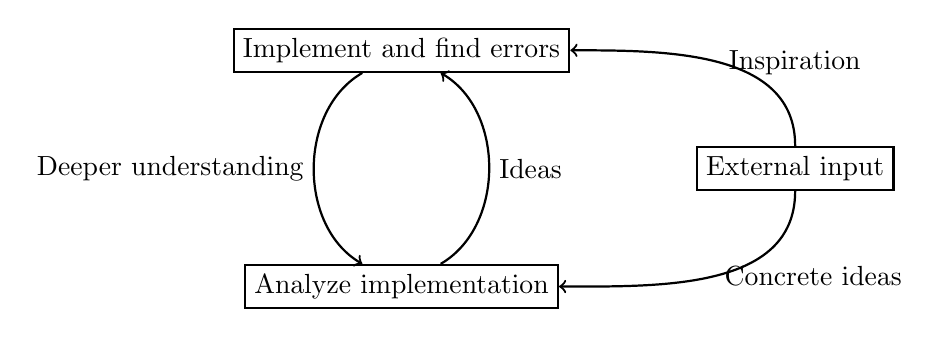
\begin{tikzpicture}[thick, node/.style = {draw}]
  \node[node] (a) at (0,0) {Analyze implementation};
  \node[node] (b) at (0,3) {Implement and find errors};
  \node[node] (c) at (5,1.5) {External input};

  \draw[->, align=left] (a) to[out=30,in=-30] node[right]{Ideas} (b);
  \draw[->, align=left] (b) to[out=-150,in=150] node[left]{Deeper understanding} (a);
  \draw[->] (c) to[out=-90,in=0] node[right]{Concrete ideas} (a);
  \draw[->] (c) to[out=90,in=0] node[right]{Inspiration} (b);
\end{tikzpicture}
\caption{The creative process of solving complex problems according to the author.}
\label{figCreativeProcess}
\end{figure}
\end{center}


% results.tex
\chapter{The Development Process}
\label{cha:Results}
The problem of doing wordlength inference is a complex problem. This section contains a series of different implementations that failed in various ways, only the last one implementation ''worked'' and is described in Section \ref{sec:Seven}.

Each section describes the thought process, implementation details of most important, new insights gained from this work and an evaluation of the final state of the implementation for each attempted solution. Explicit commit hashes are given to make it very clear what version is discussed.

\section{Inital Requirements}
\label{sec:initalReq}
Starting the implementation work we knew parts of what we wanted to achieve. We wanted a more sophisticated version of wordlength inference that handled mathematical expressions and required less manual intervention for wordlengths when writing Spade programs. The first step was understanding what was currently happening with the wordlength inference and where the problems where located. The goal of this implementation was to find out just how much we did not know about the problem of a more sophisticated wordlength inferrer.

\begin{figure}
\begin{enumerate}
    \item Require fewer explicit \verb|sext|, \verb|zext| and \verb|trunc| specified by the programmer
    \item Make it easy to support unsigned integers -- which is something the Spade compiler is hoping to add soon
    \item Be as compatible with the current mainline Spade-compiler and easily switch between different versions of wordlength inference methods such as the old and any potential improvements using AA or IA
    \item Allow for as much flexibility in language design as possible
    \item Reduce resource usage of the finished Spade program
    \item Integrate directly into the typechecker
\end{enumerate}
  \caption{A list of design requirements for improved wordlength inference}
  \label{figReq}
\end{figure}

The initial idea for requirements are listed in Figure \ref{figReq}. These requirements are prioritized so that requirement 1 is the most important and requirement 6 is the least important. The final implementation met all of the requirements except for 6 -- since the wordlength inference was implemented in a module that operates on a typechecked syntax tree.

Replacing the type inference in the current compiler with something more powerful could potentially be the best solution. The current type inference was regarded by some contributors as magic and was hard to work with and reason about -- in some sense the module was questionable technical-debt. This poses a lot of language design questions, questions this thesis hoped to avoid since it might cause features to not be merged and made useful in the mainline compiler. Considering for example that a more powerful type inference might not be desirable in the language, since with power comes complexity and more powerful typechecking-systems like Haskell, PureScript or Coq (one need only take a walk on the lambda cube from Section \ref{sec:lambdaCube}. The more complex typesystems are know to make the problem of error messages harder -- the antithesis of Spades goal of friendly error messages -- but these more sophisticated typesystems offer great benefits to those who can wield them. To add more complexity and power to the typesystem is not a change to be made eagerly.

A separate wordlength inference module is not a completely obvious solution. Splitting the wordlength inference from the typecheckeer has both pros and cons, since the information from the wordlength inference has to end up in the inferred types from the type inference the modules need some kind of communication and this communication is obviously easier if the modules are the same module. However the wordlength inference requires information about the expressions and variables used in them, which the type inference currently throws away. Wordlength inference might also be helpful for the compile-time integers that exist in Spade -- splitting the wordlength inference to a different module reduces the coherence. A few developmental excursions were made into potential easier solutions.

\section{Taxonomy of the Solutions and a Brief Overview}

\begin{figure}
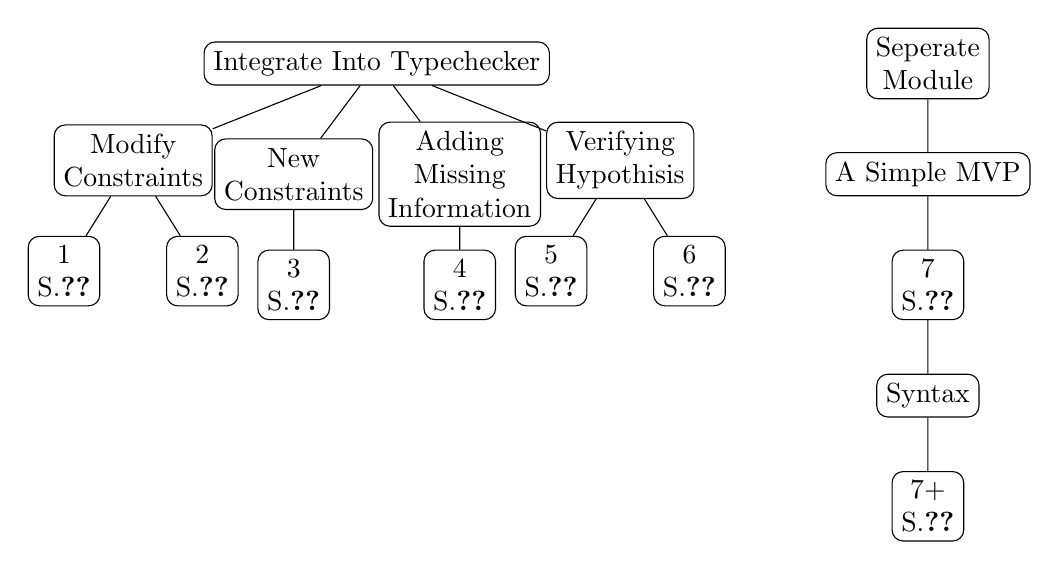
\begin{tikzpicture}[
  sibling distance=5em,
  level distance=4em,
  every node/.style = {shape=rectangle, rounded corners, draw, align=center}
]
  \node[xshift=-1cm] {Integrate Into Typechecker}
          child[xshift=-1.3em, yshift=0.5em] {node {Modify\\Constraints}
            child {node {1\\S.\ref{sec:First}}}
            child {node {2\\S.\ref{sec:Second}}}
          }
          child[xshift=-0.5em] {node {New\\Constraints}
            child {node {3\\S.\ref{sec:Third}}}
          }
          child[xshift=0.5em] {node {Adding\\Missing\\Information}
            child {node {4\\S.\ref{sec:Forth}}}
          }
          child[xshift=1.3em, yshift=0.5em] {node {Verifying\\Hypothisis}
            child {node {5\\S.\ref{sec:Other}}}
            child {node{6\\S.\ref{sec:Other}}}
          } ;
  \node[xshift=6cm] {Seperate\\Module}
          child {node {A Simple MVP}
            child {node {7\\S.\ref{sec:Seven}}
              child {node {Syntax}
                child {node {7+\\S.\ref{sec:Seven2}}}
              }
            }
          };
\end{tikzpicture}
  \caption{A overview of the different solutions and how their ideas relate to eachother -- the ideas are numbered and the relevant section for each chapter is mentioned.}
  \label{fig:taxonomy}
\end{figure}

There were a lot of implementations that were tested and iterated upon as can be seen in Figure \ref{fig:taxonomy}. The majority of attempts hoped to modify the existing typechecker into doing the wordlength inference better -- but these changes interfered with a lot of other language features like type level integer constants which are required memories. After numerous attempts it was decided to try something new from a different perspective. A seperate module for wordlength inference worked wonders and was simpler to implement, the changes are discussed further in Section \ref{sec:Seven}.


Most of the implementations from Figure \ref{fig:taxonomy} were experiments and were not thought to be the solutions most likely to work. The more encompassing and maybe easier solutions have always been adding a separate module for wordlength inference -- in a similar way to how the linear types are checked in Spade at the moment -- or adding a whole new type inference and type checker.


\section{The First Implementation -- Naive}
\label{sec:First}

It was not immediately obvious how affine arithmetic would fit into the current typesystem in Spade. What did seem like a good idea at the time was adding ranges into the integers in the typesystem. So the initial naive implementation used the \verb+ConstraintExpr+ that existed for compile time integers and tried to force it into doing better wordlength inference. \verb+ConstraintExpr+ was the basis for the current wordlength inference which simply added one to each number and was therefore what immediately sprang to mind. 
\cprotect\footnote{The changes for the first bash at the problem are placed on the git-branch \verb+the-simplest-implementation+ and has git-hash \verb+74c966a0317aa738017d2edf15def4719fe8dc95+.}

% After poking some more two different ways of expressing constraints and requirement were found \verb+ConstraintExpr+ and \verb+Requirement+. These very similarly named concepts are very similar. \verb+ConstraintExpr+ is used primarily for compile-time integers and has support for addition, negation, constants and logarithms. \verb+Requirement+ adds information that does not fit neatly into a Damas-Hindley-Milner typesystem, namely: fields a type is expected to have, methods a type is expected to have and if a type can hold a given integer literal. Both \verb+Requirement+s and \verb+ConstraintExpr+s are removed after they are satisfied for a type.

\verb+ConstraintExpr+s was hijacked it into supporting ranges, to see where the compiler started to complain and find other potential pot holes or errors. \verb+ConstraintExpr+ was changed to support addition, negation, and multiplication and operate on ranges with a a high and a low value -- in contrast to how \verb+ConstraintExpr+ worked only a single value prior. The typechecking of binary expressions was also changed to add these new kinds of constraints and checks.

This change broke a lot of things in the compiler in interesting ways. Array lengths no longer worked since they also used these kinds of \verb+ConstraintExpr+. The types of some expressions also failed to infer which caused the \verb+HIR-lowering+ to fail. The reason for the missing types was because there are choices to be made when typechecking some expressions, what wordlength should actually be used when there are multiple candidates. There was also an attempt at mitigating the missing types by introducing an extra solver stage for the \verb+ConstraintExpr+s -- this stage ran after a function was typechecked and tried to pick the smallest size of all constraints and did not work.

The change was also too large to allow as much compatibility as possible with the mainline compiler, broke language features and added more complexity to the constraint system. These changes signaled that changing the \verb+ConstraintExpr+ to operate on ranges would be too much to ask if one wanted any kind of backwards compatibility. The problem of failing to infer the wordlengths for some integers was also noted here, and that it usually was the symptom of not giving the typesystem enough information to deduce all wordlengths -- the seperate solver did not help it either.

How affine arithmetic could be added into this kind of code was still to be decided, since the typechecker is a logical system it has to run backwards which is something affine arithmetic cannot do.

The implementation outlined here did not work -- it was also never expected to work. It gave very clear hints as to where to dig deeper, where the understanding was sub par and some of the hidden requirements for adding wordlength inference.

\section{The Second Implementation -- Another Naive Stab}
\label{sec:Second}

Full with unmotivated optimism the \verb+ConstraintExpr+ was extended to support a \verb+BitsToRange+ -- which worked as the opposite of the \verb+BitsToRepresent+ expression. \verb+BitsToRange(X)+ turned a wordlength into the maximum positive value representable for a signed integer with \verb+X+ bits. The idea was to allow moving between wordlength and a max-value in the type-level expressions. This would hopefully leave the array code working, while allowing the expression code to infer wordlengths since this would be more information. An attempt at fixing the problems outlined in the first solution. This idea and implementation was not supposed to solve the entire problem completely. The second attempt was not a fit solution for the entire problem since it only solves the sub-problem of very naive interval based wordlength inference -- affine arithmetic was nowhere to be seen as mentioned. The ambition was to solve the easiest parts of the problem first since if the idea cannot handle the easy parts it is not worth thinking about the hard parts.
\cprotect\footnote{Changes are available on the git-branch \verb+the-second-simplest-thing+ and has git-hash \verb+3d92c0e4b28b64104f700c3d299f62e7938cb016+.}

\begin{figure}
\begin{minted}[linenos]{python}
def CheckAddition():
  Constraint(Result = R(M(Lhs) + M(Rhs))
  Constraint(Lhs = R(M(Result) - M(Rhs))
  Constraint(Rhs = R(M(Result) - M(Lhs))

def CheckIf():
  Unify(True, False)
  
\end{minted}
  \cprotect\caption{Psuedo code for the wordlengths of the 3 unknowns in an addition (the result, the left hand size (LHS) and the right hand side (RHS). Another function is sketched for checking of If-Expressions where \verb+True+ and \verb+False+ are the types of the results of the respective branches. \verb+ToRepresent+ is the same as \verb+BitsToRepresent+ and \verb+M+ is the same as \verb+BitsToRange+ -- the names were changed to make it easier to read at a glance. \verb+Constraint+ signals a new constraint that should be added.}
\label{fig:SecondAlgo}
\end{figure}

The Figure \ref{fig:SecondAlgo} contains pseudo code for the changes introduced in this second idea. It adds 3 constraints for an addition and 1 unification for an If-Expression. Now let us ponder the case where we have the following if-expression \verb!if ... { a } else { a + 4 }! in a context where \verb+a+ is an integer of wordlength 1 (\verb+a: int<1>+). We unify both If-branches, which causes \verb+a+ to be part of the result and the \verb+Lhs+. We can infer \verb+Lhs=1+ and \verb+Result=1+, which changes the first constraints to \verb+1 = R(M(1) + 4)+. This constraint gives a contradiction which shows how inflexible this solution is. Ideally this piece of code would compile fine -- since we can easily fir $a + 4$ into the same wordlength as $a$. But to get this to typecheck we require a \verb+sext+, which highly contest out first requirement.

The constraints listed in \ref{fig:SecondAlgo} are all equality-constraints (\verb+=+) and for this idea to work less-than-or-equal constrains (\verb+<=+) would be more suitable. Less-than-or-equal constraints might be required for wordlength inference, but these cannot be expressed in the Spade typsystem as is. The problem of adding affine arithmetic is still unsolved. We want to encode the operations and additions into a structure to support affine arithmetic -- which would then require a new system to work in parallel to . We also need to carry the information for the intervals of variables somewhere else, since the current typesystem really disagrees with encoding ranges into int-types -- a new construction is required. 

\section{The Third Implementation -- Considering Equations}
\label{sec:Third}
The third attempt focused on adding equations and added a separate constraint language. These constraints are part of the type inference.
\cprotect\footnote{Changes are available on the branch \verb+the-third-simplest-with-equations+ with the git-hash \verb+ 83d1da48f5010767b9a96aea0a5bca13b7415084+.}

A new set of constraints was added giving \verb+ConstraintExpr+ and \verb+Requirement+ a new friend called \verb+SizeExpression+. Aside from the obvious technical-debt with 3 different kinds of constraints that express similar ideas -- the solution was deemed too ''ugly''. The constraints needed for \verb+SizeExpression+ were required to be feed forward by the type inference -- following a completely different approach to the other requirements which were added to lists. This caused a large amount of changes in the type inference which was preferably to be avoided.

We also start to suspect that the wordlength inference might \textit{need} to be a separate module, split up from the type inference and run after all the types have been inferred. This idea did however not live long, and might even be a mere curiosities.

\section{The Fourth Implementation -- A Desperate Attempt}
\label{sec:Forth}

Almost out of desperation for getting something to work. Just to make sure this whole ordeal wasn't impossible -- these changes were made. These changes are also the most insightful in all of these experiments.
\cprotect\footnote{The changes are available on the git-branch \verb+the-fourth-attempt-now-with-equivelence+ and has git-hash \verb+ba0fa1baab56a725c31f703204da3b7d5f44380a+.}

\begin{figure}
\begin{minted}[linenos]{python}
CheckAddition():
   # Take our best guess of a max value
   LhsMax = PassedLhsMax or Largest(LhsSize)
   RhsMax = PassedRhsMax or Largest(RhsSize)

  # We know the maximum values add to give a new maximum
  Constraint(ResultMax = LhsMax + RhsMax)
  # The maximums implies a size for each of the values
  Constraint(ResultSize = ToRepresent(ResultMax))
  Constraint(LhsSize = ToRepresent(LhsMax))
  Constraint(RhsSize = ToRepresent(RhsMax))
  # Return our best guess to make the expressions around aware of us
  return ResultMax
\end{minted}
  \cprotect\caption{Psuedo code that described the idea for inferring wordlengths with extra information -- what was used in the fourth attempt. Here \verb+PassedLhsMax+ and \verb+PassedRhsMax+ are type variables that sometimes exist and are results of typechecking similar expressions -- one can envision some code that calls \verb+CheckAddition+ for each of the subexpressions in the binary expression we check addition for. \verb+ToRepresent+ convert a maximum value to the smallest wordlength that can fit it. \verb+Largest+ is almost the opposite of \verb+ToRepresent+ and change a value to the maximum value such a wordlength can hold}
\label{fig:psuedoFour}
\end{figure}

The psuedo code in Figure \ref{fig:psuedoFour} describe how an addition expression is wordlength inferred according to the fourth method. The code sent extra information -- besides of the wordlength stored in the type of each integer. This extra information also resulted in extra type variables which denoted the maximum value -- these type variables could not be explicitly manipulated and where hidden from the user of the language. These type variables were not strictly bound to anything and were hard to reference since they could not be found from the type they were constrained to if the constraints were satisfied and thus discarded. There was not a problem with the kind or number of constraints since \verb+LhsMax+ and \verb+RhsMax+ was always known or bound directly to a size.

This was the first approach to produce better wordlength inference and handled expressions such as \verb!a + 1 + 1! as one would expect by not increasing the wordlength by 2 but by 1 when the type of \verb+a+ was larger than 2. There is also a very concrete way to introduce negative ranges -- just add another type variable. This means the solution clearly solves the requirements 1, 2, 3, 4 and 6 from Figure \ref{figReq} -- the resource usage was never investigated.

This solution also introduced problems with the hidden type variables. Since the type variables for the maximum size cannot be referenced in any meaningful way from the type of the expression it was deemed be difficult to explain to the user of the language why a type-conclusion was reached. But since constraints were discarded after they were satisfied the relations between the type variables and the maximum size was also discarded -- this meant that range information could not be recovered. The problem of integrating AA was not prodded in since this solution was not good enough -- due to the potentially unsatisfactory error messages. The problem with equality constraints (\verb+=+) from Section \ref{sec:Forth} is also relevant, since it might force a value to have multiple wordlengths -- a neater solution is still less-than-or-equal constraint (\verb+<=+).

\section{Other Implementations -- Just Curiosities}
\label{sec:Other}

There were two more attempts at an implementation inside the type checker. Both these experiments yielded little of interest since they mostly verified the previous claims, mostly the implementations from Section \ref{sec:First} and Section \ref{sec:Second}. They were also very shallow changes since the more promising change outlined in Section \ref{sec:Seven} was started on instead. These ideas mainly focsed on re-testing old ideas and are of little interest for the final results.
\cprotect\footnote{Available on the git-branches \verb+the-fifth-attempt-now-without-returns+ and \verb+the-sixth-attempt+}

%%%%%%%%%%%%%%%%%%%%%%%%%%%%%%%%%%%%%%%%%%%%%%%%%%

\section{The Seventh Implementations -- a Separate Module}
\label{sec:Seven}
After doing a lot of thinking and reasoning we decided to see how a separate module would look -- in theory this would give maximum flexibility in how the wordlength inference worked. Using a separate module for the wordlength logic also meant changing it in the future would be easier, if more experiments would be conducted.%
\cprotect\footnote{Changes are available on the branch \verb+the-seventh-attempt-almost-as-simple-as-attempt-one+ with git-hash \verb+889afd61a59f04f60730964b8ae7a2703110dd99+, these changes were merged and is available in the PR hosted on \url{https://gitlab.com/spade-lang/spade/-/merge_requests/200}.}%
Since the type checker would not be changed as much old programs could still be compiled and thus compared with and without the more advanced wordlength inference.%



As a basis for the wordlength inference there is a simple type called \verb+Range+. \verb+Range+ can be directly mapped to the interval from IA. The datatype is implemented using \verb+BigInt+ to make sure no wrapping occurs. There is also a type called \verb+AAForm+ which maps directly to the form of AA expressions -- \verb+AAForm+ is implemented as variables and constant scalars which are \verb+BigRational+s. The decision of using \verb+BigRational+ was to avoid even more noise in the AA implementation.


\begin{figure}
\begin{minted}[linenos]{python}
def Visit(Construct):
  Constraint = match Construct:
    # Variables are already resolved so we just need to make sure the inference
    # has id's that match 1:1 with the typechecker.
    case Var(VarId):
      if VarId not in KnownVariables:
        KnownVariables[VarId] = GenerateNewId()
      KnownVariables[VarId]

    # Constants are simply the constant, the range of these are known here.
    case Constant(Constant):
      RangeFromConstant(Constant)

    # Constants are simply the constant, the range of these are known here.
    case Assignment(Var, Expr):
      Constraints[VarId] = Visit(Expr)
      NotAnExpression

    # Binary expressions need to be recorded, we want to build up a complete
    # list of the constraints for each type.
    case BinaryExpr(Op='+', Lhs, Rhs):
      Addition(Visit(Lhs), Visit(Rhs))
    case BinaryExpr(Op='*', Lhs, Rhs):
      Multiplication(Visit(Lhs), Visit(Rhs))

    # Uniary expressions also need to be encoded.
    case UnaryExpr(Op='-', Operand):
      Negation(Visit(Operand))

    # Flow control constructors need to be handled differently, for an If we #
    # combine them and realize that the result must lie inside the union of both
    # branches - we return either True or False but we cannot know which for
    # all cases.
    case If(Condition, True, False):
      Visit(Condition)
      Union(Visit(True), Visit(False)

  # Register this constraint, since *all* expressions have types we want as
  # many constraints as possible.
  Constraints[Construct] = Constraint
\end{minted}
  \caption{Psuedo code for visiting the entire syntax tree -- some details have been omitted. The algorithm handles each node separately and visits all the inner nodes, taking care to visit \textit{every} expression in the syntax tree and accumulating constraints for the types they relate to.}
\label{fig:AstWalker}
\end{figure}


The idea for the implementation was to walk the entire AST a second time after typechecking had run and monomorphisation was completed -- each entity was given to the wordlength-inference module\cprotect\footnote{The wordlength-inference module was called \verb+spade-wordlength-inference+} -- this built up constraints described in the algorithm from Figure \ref{fig:AstWalker}. The algorithm makes sure to visit \textit{every} expression in the AST and record down their relation to each other and since we have already typechecked we know which expressions need to constraints built up. The algorithm in Figure \ref{fig:AstWalker} produces a mapping between language constructs and constraint equations relating it to expressions that have a relation. This mapping is almost what we want, and we can use it to produce the mapping from a type variable and an equation which describes the expressions size as related to other expressions. We can of course have multiple equations for the same type variable as long as they are consistent with each other. After all of these constraint equations have been gathered up we can pass the equations onto a solver. 

\begin{figure}
\begin{minted}[linenos]{python}
if InferMethod == OLD: return

# Here we call `Visit` internally to visit all the relevant expressions, we get
# out a mapping from type variables to equations.
(Variables, Equations) = VisitAllIntegerExpressions(AST, TypeChecker)
# We can also ask the typesystem for the sizes it has deduced, since we may not
# disagree with the typechecker. A mapping from typevariables to their known size,
# we will fill this in with more information as we proceed.
Known = ExtractKnownWordlengths(Variables, AST)

for _ in Equations:
  KnownAtStart = Known
  for (Var, Body) in Equations:
    MaybeValue = case InferMethod of
                  IA -> EvaluateUsingIa(Known, Body)
                  AA -> EvaluateUsingAa(Known, Body)
    match MaybeValue:
      Just Value -> InjectAndCheckForContradictions(Value, Known)
      Nothing -> pass
  # If we did not progress we abort
  if KnownAtStart == Known:
    break

for Var in Variables:
  unify(TypeChecker, Var, Known[Var])
\end{minted}
  \cprotect\caption{The algorithm used in the seventh attempt to determine the wordlength for all expressions in a spade-program. \verb+VisitAllIntegerExpressions+ visits all the integer expressions in the AST with some help from the typechecker state and returns a set of all type variables mentioned in an equation and a list of tuples containing type variables and the requirements posed from their wordlengths.}
\label{fig:WLIAlgo}
\end{figure}

The algorithm from Figure \ref{fig:WLIAlgo} has a runtime of $O(n^2*d)$ where $n$ is the number of equations and $d$ is the largest depth of the equations -- since we are bounded by running the loop a maximum of $n$ times. Though average runtime is significantly better since it can solve most sets of equations efficiently in fewer iterations. If the algorithm can make progress we also know that it will, since it evaluates all equations for each pass -- this is a form of breath first search since we constantly re-check the equations and disallow variables to shrink in size we always find more information with each iteration.

The inference algorithm from Figure \ref{fig:WLIAlgo} can be applied from the constraints gathered from the algorhtm in Figure \ref{fig:AstWalker}. This means we've visited the entire AST, picking out the expressions that are typed to be \verb+int<_>+ and construct algebraic constraints on the form \verb+<var> = <expression>+. We can then feed these equations into a solver and use them to solve more equations -- here we can pick between using using IA or AA. In the implementation this could be set when running the compiler \cprotect\footnote{The different wordlenght inference options could be swapped using the environment variable \verb+SPADE_INFER_METHOD+, the inference logic could also be disabled entirely, this was required since the Swim buildsystem is very peculiar about the flags passed to the compiler.}. We can then enrich the typecheckers types with our new findings which lets us reuse the rest of the compiler tool chain -- very nifty!

\subsection{Evaluating the Changes}
This implementation of the spade compiler was then run on the example program \verb+spade-memory-display+ using the swim command \verb+SPADE_INFER_METHOD=XX swim pnr+. A simple bash script was made to record the number of LUTs used in the FPGA when the command was executed and this was stored in a file. The program was compiled 50 times for the three configurations: ''Old Mode'' -- denoted by ''ONE'', ''Affine Arithmetic'' -- denoted by ''AA'', ''Interval Arithmetic'' -- denoted by ''IA'', the number of LUTs used was then feed into a spreadsheet program and produced the table in Figure \ref{fig:SpadeCompilations50Table}.

\begin{figure}
\begin{center}
\begin{tabular}{l | c c c}
  & ONE (Old version) & IA & AA \\
\hline
Average number of LUTs&179.6&176.9 & 177.1 \\
Variance for number of LUTs &13.2&6.0&8.2 \\
Largest number or LUTs&186.0&181.0&183.0 \\
Smallest number of LUTs&171.0&171.0&167.0 \\
\end{tabular}
  \caption{The number of LUTs after PNR for the project spade-memory-display with different versions of wordlength inference in table form.}
  \label{fig:SpadeCompilations50Table}
\end{center}
\end{figure}


Figure \ref{fig:SpadeCompilations50Table} shows a slight decrease in variance for the number of LUTs generated using ''IA (Interval Arithmetic)'' and ''AA (Affine Arithmetic)''. The average stays almost the same for all methods with ''ONE (The Old Version)'' being a bit higher than the others -- but not by a statistical margin.

\begin{figure}
\begin{minted}[linenos]{rust}
// Old spade wordlength inference
fn add_and_subtract(x: int<5>) -> int<11> {
  (x - x) + (x - x) + (x - x)
}

// New spade wordlength inference using AA
fn add_and_subtract(x: int<5>) -> int<0> {
  (x - x) + (x - x) + (x - x)
}

// New spade wordlength inference using IA
fn add_and_subtract(x: int<5>) -> int<8> {
  (x - x) + (x - x) + (x - x)
}
\end{minted}
  \caption{A simple spade function showing the difference in the wordlength inference with the new approaches with a focus on addition and subtraction.}
  \label{fig:CodeThatWorksNow}
\end{figure}

These changes did shown promise in the usability of the language. Snippets like the one shown in Figure \ref{fig:CodeThatWorksNow} were typechecked a lot better by the spade compiler and in that sense a usability improvement can be seen, note especially the difference in the return type of the function \verb+add_six_times+ where the one typechecked with ''Affine Arithmetic'' always returns 0 and ''Interval Arithmetic'' returns 8 bits -- compared to the ''Old'' approach which returns an integer with 11 bits. % The number of cases where a frivolous truncation was needed has decreased due to these changes. This can lead to clearer and more concise code.


This implementation leaves a gaping hole roughly the size of an elephant. How does a user of the Spade language define these ranges? Since the changes discussed until now have not touched the syntax or the type checker (except disabling the old wordlength inference), the entire language as a whole is completely blind to the ranged-based wordlength inference. The current approached seemed to work well and it was decided that the best course of action was to extend this implementation.

\section{The Seventh Implementation Extended -- Doubling Down on Ranges}
\label{sec:Seven2}
After the success of the implementation in Section \ref{sec:Seven} more work was needed to communicate the intended ranges from a programmer, thus began changes that updated the syntax and the typechecker in Spade to supportrange. There was however a previous attempt at adding this kind of range syntax and are available in the Spade git-lab\cprotect\footnote{\url{https://gitlab.com/spade-lang/spade/-/merge_requests/208}} that focused on the syntactical changes and avoided the typesystem changes, the merge request has since been abandoned. The new changes that needed to be made to the syntax took inspiration from the previous attempt.
The new syntax and typesystem changes had to be scoped accordingly and a lot of the details and changes discussed are very opinionated and this thesis tries to not focus too closely on the design of programming languages and more on the actual implementation of the language features, though some background and reason will of course be given. \cprotect\footnote{Changes that are available in the git-branch \verb+wordlength-inference/push-the-changes-further+ with git-hash \verb+ee9980c6ec518dbdf0794dbb9193c5b1c9b6945e+} 

The previous attempt at changing the wordlength syntax tried to work from the syntax forward without interfering with the typesystem -- this was deemed to be harder than expected. This new attempt tried to change both the syntax and the typesystem at once -- this proved to be beneficial but the change was also quite large and caused a large break in the syntax and semantics of the Spade language. Basing the range based syntax on the newly implemented wordlength inference simplifies a lot of details.

\begin{figure}
  \begin{minted}[linenos]{rust}
fn twice<#A, #B, #M, #N>(x: int<A..B>) -> int<M..N> {
  2 * x
}

fn add_one<#A, #B, #M, #N>(x: int<A..B>) -> int<M..N> {
  x + 1
}

entity main(clk: clock, rst: bool) -> int<14..14> {
  let a: int<6..6> = twice(3);
  let b: int<7..7> = add_one(a);
  let c: int<14..14> = twice(b);
  c
}
  \end{minted}
  \caption{A small spade program that shows the new range syntax in context and gives an example of how integer range information is now more detailed.}
  \label{fig:BetterProgram}
\end{figure}

The syntax of the Spade language was first of all changed to parse \verb+int+ types differently, the syntax \verb+int<L..H>+ allowing ranges to be specified. The old syntax \verb+int<W>+ was still supported but was syntactic-sugar for \verb!int<!$-(2^{w+1})$\verb!..!$(2^{w+1})-1$\verb!>! (the $+1$ part comes from all integers being signed in Spade) since this would give partial compatibility with older spade-program. In the previous work a lot more syntaxes were added but they were questionable extraneous for updating the type inference. This change makes it possible to propagate the range information from one function to another in the form of a range -- which is more precise than a wordlength which was what was available before. The Figure \ref{fig:BetterProgram} shows this new syntax in a small example spade-program. The extra variables \verb+a+, \verb+b+ and \verb+c+ are required to make the program compile, since the compiler has trouble typechecking the variables between the expressions, this is a problem of the unification process and that there are insufficient requirements on some generics.

It is also worth noting that the extra types in on lines 10 to 12 in Figure \ref{fig:BetterProgram} can be larger according to the current rules -- but must include the constants defined there.

The \verb+int+ type also had to change to work with 2 generic arguments -- a lower and a higher bound. These types had to be inserted in the type checker. Making this change in full would require rewriting almost every single spade-compiler test, and would be a substantial amount of work and time, more time than this thesis has been allotted. The decisions to break with the best practices of software development was taken to make sure the thesis could be finished at all. Some of the tests were fixed where it was deemed simple to do so. Most of these changes were very mechanical though. The wordlength inference code also needed to be changed slightly to accept the new ranges as inputs from the type checker.

These changes also made the type checker aware of the range based semantics of integers in the wordlength inferrer -- thus the type checker could be used to propagate type information about these ranges. This made all library functions which previously only used wordlengths work properly with arbitrary range. Users of the spade language could now also specify ranges on their types themselves.

An extensions was also made to the wordlength inference methods described in Section \ref{sec:Seven}. A naive method that runs both ''Interval Arithmetic'' and ''Affine Arithmetic'' and returns the subset was also introduced.

The very basic implementation in this thesis does not handle memories and registers. Though supporting them should be very minor work, but requires a lot more verification. There are also questions as to the language features of registers and memories should interact with the range-based syntax of integers. The unification rules from the type checker are also very strict and disallow things like passing a constant to a function that takes an integer argument that is not constant. How these problems are to be solved is according to the thesis authors a matter of taste, though these problems do exists and needs addressing. 

\subsection{Evaluation the Changes}
After a change has been made it needs to be verified and tested. A custom version of the compiler with the changes described in Section \ref{sec:Seven2}. Each program was PNRd 51 times for each of the three configurations ''AA'', ''IA'' and ''AAIA'' -- and a clean of the build environment was conducted between all steps. The changes breaks a lot of compatibility with older Spade-versions which severely limits the number of Spade programs that can be used since a dependency written for a different version of the compiler is not going to compile.

\subsubsection{spade-memory-display}
The small library \verb+spade-memory-display+ was used for evaluation. The changes to the compiler required changes to the library code in order to compile, this made it unclear how to compare directly with older versions of the compiler since small code changes can have large changes in the output. The library code was PNRd 51 times for each of the three configurations ''AA'', ''IA'' and ''AAIA'' with \verb+swim clean+ ran between each build.
 
\begin{figure}
\begin{center}
\begin{minted}[]{text}
ICESTORM_LC: 190/1280 (14.8%)
ICESTORM_PLL: 0/1      (0.0%)
ICESTORM_RAM: 0/16     (0.0%)
SB_GB: 2/8            (25.0%)
SB_IO: 4/112           (3.6%)
SB_WARMBOOT: 0/1       (0.0%)
\end{minted}
\end{center}

  \caption{The output from every place and route run given regardless of wordlength inference method for the spade-library spade-memory-display.}
  \label{fig:SMDoutput}
\end{figure}

All builds produced the same metrics and is presented in Figure \ref{fig:SMDoutput}. The metrics shows no difference for any of the 153 place and route compilation of the spade-library. All of the compilations used 190 LUTs. 

\subsubsection{A Simple FIR-filter}
FIR-filters are often implemented in hardware since they are of great use for signal processing in general. So a simple FIR-filter program with 100 elements was setup. The code was PNRd 51 times for each of the three configurations ''AA'', ''IA'' and ''AAIA'' with \verb+swim clean+ ran between each build. The FIR-filter program in its entirety is available at \href{https://github.com/FredTheDino/thesis-spade-lang/tree/main/messing/fir}{https://github.com/FredTheDino/thesis-spade-lang/tree/main/messing/fir}.

\begin{figure}
\begin{center}
\begin{minted}[]{text}
ICESTORM_DSP: 0/8    (0.0%)
ICESTORM_HFOSC: 0/1  (0.0%)
ICESTORM_LC: 2/5280  (0.0%)
ICESTORM_LFOSC: 0/1  (0.0%)
ICESTORM_PLL: 0/1    (0.0%)
ICESTORM_RAM: 0/30   (0.0%)
ICESTORM_SPRAM: 0/4  (0.0%)
IO_I3C: 0/2          (0.0%)
SB_GB: 0/8           (0.0%)
SB_I2C: 0/2          (0.0%)
SB_IO: 13/96        (13.5%)
SB_LEDDA_IP: 0/1     (0.0%)
SB_RGBA_DRV: 0/1     (0.0%)
SB_SPI: 0/2          (0.0%)
SB_WARMBOOT: 0/1     (0.0%)
\end{minted}
\end{center}

  \caption{The output from every place and route run given regardless of wordlength inference method for the simple FIR-filter.}
  \label{fig:FIRoutput}
\end{figure}

The Figure \ref{fig:FIRoutput} shows the output from every PNR run for the FIR-filter program. All the outputs were identical regardless of what wordlength inference method was used. It is also worth noting that for ''IA'' and ''AAIA'' the return type of the \verb+fir+-function can be simplified to \verb+int<0..1000000>+. The return type is required to be \verb+int<-500000..1000000>+ for ''AA'' which goes into the negative even though it cannot possibly happen.

\subsubsection{Comparing The Ranges For Simple Expressions}
The wordlength inference was also compared on 3 expressions: $a - a + a - a + a - a$, $(a - b) \cdot (b - a)$ and $a \cdot a \cdot b \cdot b \cdot c \cdot c$, for all of the 3 methods ''AA'', ''IA'' and ''AAIA''. All arguments had a wordlength of $5$ and of the range $0..100$ the resulting range was noted in the table in Figure \ref{fig:CompareThings}.

\begin{figure}
  \centering
  \begin{tabular}{l | c c c}
                                    & IA     & AA     & AAIA    \\
                                    & \multicolumn{3}{c}{Wordlength $= 5$} \\
    \hline
    $a - a + a - a + a - a$   & $-93..93$ & $0..0$          & $0..0$       \\
    $(a - b) \cdot (b - a)$             & $-961..961$ & $0..0$           & $0..0$       \\
    $a \cdot a \cdot b \cdot b \cdot c \cdot c$         & $-15728640..16777216$      & $-16794692..16794693$      & $-15728640..16777216$ \\[0.7em]
                                    & \multicolumn{3}{c}{Range $= 0..100$} \\
    \hline
    $a - a + a - a + a - a$   & $-300..300$ & $0..0$          & $0..0$       \\
    $(a - b) \cdot (b - a)$             & $-10000..10000$ & $0..0$           & $0..0$       \\
    $a \cdot a \cdot b \cdot b \cdot c \cdot c$         & $0..10^{12}$      & $-9.6875^{12}..10^{12}$      & $0..10^{12}$
  \end{tabular}

  \caption{A table showing how different wordlength inference methods compare on simple mathematical expressions where all variables have the word length of 5 or are in the range 0 to 100.}
  \label{fig:CompareThings}
\end{figure}

The table in Figure \ref{fig:CompareThings} shows that ''AAIA'' always produced the tightest ranges. The last multiplication test on the third row also shows an example expression where ''IA'' produces a tighter range than ''AA''.




% discussion.tex
\chapter{Discussion}
\label{cha:Discussion}
After a thorough evaluation of the different suggested methods of implementing wordlength inference the implementations and their evaluations are discussed. Much of the discussion focuses on the final implementation since it produced the best results and was subject to the most evaluations.

\section{Results}
The Spade compiler was successfully changed to support ranges and more sophisticated wordlength inference. These changes were not able to be completed to the degree that they could be fully integrated into the mainline compiler -- but most of the technical problems have been solved. What remains are language design decisions and glue code.

The table in Figure \ref{fig:CompareThings} shows that the AAIA method results in the thightest ranges and the smallest wordlengths. That a combination of the techniques is superior is hardly surprising since IA handles multiplication better for expressions with a 0-lower bound while AA can handle subtractions of the same constants. A combination is bound to work better than any of them in isolation. Of special consideration is how IA handles $0$ a lot better, since ranges bound by 0 are still bound by $0$ even after multiplication, this is not the case for AA. This begs the question if there is a better method that would give even tighter ranges, and might be a suitable future work.

The internal changes to the Spade compiler type inference caused a sea of troubles to appear. If the Spade project want to integrate these changes fully care needs to be taken when implementing and updating language features like memories. There is also a lot of work needed to port all the tests for the Spade language. All of these are fairly manual changes but might require a lot of time. To fully integrate these changes a series of language design decisions would also need to be taken, for example how constants passed to functions should type check or the example in Figure \ref{fig:BetterProgram} which require extra help when inferring some type variables -- this is believed to come from function calls being opaque to the wordlength inference

The opaqueness of functioncalls is a large problem in the current implementation, and perhaps the simplest way of solving is probably to move the wordlength inference into the typeinference module. The information that is needed is nowhere to be found in the wordlength inference stages of the compiler and should either be rebuilt or preferably given with the type checking state. But it might also be a sign that the method described in Section \ref{sec:Forth} might have been an even better choice -- and if the typechecking were to be changed to function on ranges which was also required to change in Section \ref{sec:Seven2} there might be a better implementation that easily fits into the typechecking step of the Spade compiler.

There was no discernible difference between the PNRd programs with any of the wordlength inference methods. The table in Figure \ref{fig:SpadeCompilations50Table} motivates this -- even though the averages might suggest subtly against it. This means there is no real difference in LUTs or memories used when using the wordlength inference in this thesis. It might be claimed that the difference in variance is an improvement, it might also be due to random noise from the compiler since PNR has undeterministic behavior. Figure \ref{fig:SMDoutput} and Figure \ref{fig:FIRoutput} support the claim of little difference. Though it is worth noting that something might be different in the compilation process since both of these figures show no noise. It might be the case that these improvements only aid the more sophisticated optimization steps in the PNR-phase, and this could also explain why the improvement negligible. This might signal an error in the experiments and that the Spade implementation with the range-based wordlength inference might have a bug which causes incorrect codegeneration, unfortunately there was no access to hardware to verify this implementation on. This is a major limitation of this study but does not deter from the wordlength inference presented or the conclusions reached.

The solver for wordlengths that is described in Section \ref{sec:Seven} is very simple -- and as thus might not produce the best results possible. The solver does not handle solving equations with unknowns on both sides of the constraint, and variables being opaque to the AA method makes it produce worse results in some cases though most of the experiments in this work are simple enough to not make a huge difference. The inference algorithm could be modified to substitute entire expressions when evaluating using the AA method and it would probably produce slightly better results -- though the types would still need to be reduced to ranges.

In the Spade language wordlength inference is now more flexible, and allows propagation of ranges between functions. That wordlength information can be sent in more detail between different parts of the program means that developers need fewer assumptions of how the code works. Less assumptions result in fewer sign-extensions and truncation operations on integer expressions. The power of AA also makes it beneficial to write larger expressions instead of splitting them up in smaller chunks with placeholder variables -- since variables are always reduced to ranges by the wordlength inference algorithm for variable types.

Unfortunately the representation of integer values inside of the Spade compiler is ranges, which hinders some of the AA inference. Since each variable in Spade has a singular range paired with it the information of the sub-expressions is discarded: the information AA uses to function well is lost. For the AA wordlength inference method each variable is opaque and cannot be inspected into. Since variables are opaque it is better to inline expressions without the use of variables since the wordlength inference code can reason a lot better about those expressions.

\subsection{Limitations in the Spade Compiler}
The implementation offered in this thesis can have quite confusing error messages. This is due to the type checker discarding information of where typeinformation came from -- and the type inference module is left looking at the expressions and types given by the type checker. Changing what the Spade compiler stores from the typechecking phase would require a fair bit of plumbing but still nothing hugely complicated to implement. For later stages in the compiler it would be preferable to make some changes in the compiler to support:
\begin{itemize}
  \item A list of spans that have been unified to give a type for an expression -- this would make it possible to point to the type signatures from stages that do e.g. constant folding or wordlength inference.
  \item A full list of the constraints and requirements for a type -- currently the compiler tosses these constraints and requirements when they are deemed satisfied, this discards the sources of facts that both the type checker and wordlength inference module would find helpful.
  \item It would be great if \verb+Requirement+ and \verb+ConstraintExpr+ could be one construction -- it would aid interop and remove some technical debt in the type checker.
  \item It would also be beneficial if each entity in the Spade program could be compiled as far as possible -- so if type checking for one function of the program fails the wordlength could still be checked for an entity that is not related.
\end{itemize}

There are also profits in the area of usability of the Spade language -- removing truncation operations from the Spade code can make the code a lot more readable. Since most of the truncations and sign extensions are required by the very simple wordlength inference method present before this thesis it is probably the single largest contribution that has been made. The change in wordlength inference makes the Spade compiler more flexible and makes it possible to remove a lot of the truncation and extension operations.

\section{Method}
The method does not focus directly on wordlength inference but focuses more on the software development side, which is in stark contrast with the research questions. This might however show more fault in the usage of research questions than this thesis. The authors do believe the code changes that came from this thesis to be among the best possible for the given time. The fumbling evaluation of alternative implementations give a basis for that argument. It is however possible for such an implementation to have been found by thinking very carefully and very hard -- though theoretically sound ideas often crumble in agony when faced with the sledgehammer that is reality. Especially if those theories are drawn from inexperience.

From software development it is well known that an iterative approach to software development often yields the best results in a fixed amount of time. The idea of using some form of agile development methodology seems to have been a sound idea.

It is also frustrating to leave the compiler in a state where most of the work is \textit{almost} done. As stated earlier in the thesis -- it is possible that some of the changes that need to be done are in fact harder than they appear. But programming work is well known to be hard to plan. This thesis does however leave a good base to work further on the compiler. It might also be for the better that these other changes are made by someone on the core Spade compiler team. Though this thesis has been a collaboration with the Spade compiler team communication is always lossy, and details are bound to be forgotten. Hopefully these changes are well documented enough to be of use and be able to be well integrated into the language.

\section{The Work in a Wider Context}
More sophisticated wordlength inference in Spade unfortunately has little effect on the planet or the current war in Ukraine that is currently raging. But this contribution need not be discarded as useless. A slight improvement in efficiency for hardware designs can have cascading effects on how cheap it is to produce custom circuits. The cheaper cost can of course lead to an increased production which is what has already happened to goods such as computers and cars. Hardware description languages and FPGAs is used heavily in the weapons industry and thus code created in this thesis might contribute to more raging wars. However, it's essential to recognize that war is a double-edged sword -- it can both preserve and condemn -- yet its inherent nature remains one of destruction.

Hopefully hardware designers will rejoice over this work.


% conclusion.tex
\chapter{Conclusion}
\label{cha:Conclusion}
Programming languages are complex things -- but they need to be complex to express complex and precise ideas. The wordlength inference outlined in this thesis shows a good way to extend the Spade hardware description language to more flexibly handle wordlengths. The wordlength inference works well with the current Damas-Hindley-Milner type checker and will allow language designers of the Spade language to make an active choice in how the Spade language should interact with wordlengths. There was no difference in the resource usages of spade programs before or after the wordlength inference from this paper was introduced. The authors believe that the real benefit from these changes will not come from performance gains -- though better performance might be possible in the future -- but the ''soft'' value of expressiveness and clearer programs. A possibility of clearer intent will make it possible for the Spade compiler to more clearly understand the programmer and might make more readable code and aid optimizations.


\section{How can interval arithmetic and affine arithmetic be used to implement wordlength inference?}
The most optimal way was to combine both interval arithmetic and affine arithmetic. Since both have different strengths and weaknesses the combination of the methods costs little in the way of resources but can in some instances give a lot smaller ranges which leads to smaller wordlengths. If this work is to be extended to support unsigned integers this combined method is bound to come in very handy. 

\section{How does wordlength inference and optimization affect the number of LUTs, DPS-blocks and memories for a circuit?}
This thesis clearly shows that this implementation of wordlength inference has no discernible effect on any resource usage metrics.

\section{Can wordlength inference be used to create more reusable code?}
The final state of the changes from this thesis made the compiler very finicky about wordlengths. The expressiveness in the typesystem has increased which has made it possible to express some types more clearly and making certain function types more expressive, making functions a more well integrated language construction -- aiding the reusability of code. Though it does not aid the resuability greatly the authors claim this is an improvement no matter how modest it is. Future work could easily expand on this.

\section{Future Work}
The implementation used in this thesis opens the door for an even more sophisticated approach where sub-expressions could be evaluated by either AA or IA. One can consider an evaluation tree where all possible combinations of AA and IA are used -- though this tree might be too large to easily evaluate in practice, a technique like this would give theoretically optimal wordlengths for expressions. Removing the requirement that variables are opaque could also make the wordlength inference a lot better and might also be an interesting point of research in the future.

Since the Spade compiler now understands expressions and the values the expressions can be evaluated to it is trivial to check for expressions that evaluate to a constant. A constant expression is almost always a programmer error, but even when it isn't it should be replaced with the constant for clearer readability. This range analysis can also be used to trim dead code even before the code generation, and then warn about unreachable paths.

Since the compiler now reasons about ranges of integer values unsigned integer optimizations should be possible to do in a multitude of places. Maybe even automatically generating code that uses unsigned integers if the code never goes below 0. But this can of course be taken a step further, and all expressions could be re-written by the compiler to avoid going below 0. We can trivially rewrite the expressions inside the compiler since integer arithmetic is a well behaved ring (unlike floating point numbers). This could lead to improved resource usage in some places. Maybe it could even be possible to shift the representation of numbers inside the compiler.

Some of the typing and inference rules need to be updated to make the language work well with e.g. Constants passed to functions. Looking into these kinds of rules could make the language clearer and more expressive -- pairing it with a usability study could be very enlightening.

There are also more advanced wordlength inference methods. There are alternatives to AA which might prove useful -- like ME-gPC. Maybe it is possible to track every possible integer value an expression can take, and allowing these holes in the expressions would make it possible to give even more precise guidance and help.

Maybe it could be possible to pair the Spade-language with more complex formal verification methods, and allow formal verification of circuits in the language directly. The language for the generics could also be extended to support this formal verification step, so that constraints for functions that require certain ranges based on the input can be wordlength inferred and typechecked more seamlessly. For an example envision the type signature \verb+fn double<#A, #B>(a: int<#A..#B>) -> int<2*#A, 2*#B>+.

This work has added a separate wordlength inference module in addition to the typechecking, but it might still be very beneficial if they are one and the same -- and thus looking into more complex type systems or reworking the current typesystem might still be a good idea, this is another way to make functioncalls less opaque.

The level of improvement that is gained by this improved wordlength inference might be overshadowed by the work of the PNR tools -- as such it might be the case that we alleviate a bit of PNR work with more improved wordlength inference, this might lead to better compile times. Investigating the relationship between compiletimes and these kinds of optimizations might be very interesting.

As a personal note, I'd find it very interesting to add an interpreter to the Spade-language such that designs could be simulated without the need of an FPGA, this could also aid different kind of verification and might be an alternative to a more powerful typesystem.


\clearpage

\printbibliography

\appendix
% appendix_version_and_hashes.tex
\chapter{Versions and Hashes}
\label{app:VersionsAndGitHashes}
This section contains githashes of the Spade compiler that have been mentioned in this thesis.
All code is available at \href{https://gitlab.com/FredTheDino/spade}{https://gitlab.com/FredTheDino/spade} -- the thesis GitLab.
\begin{minted}[]{text}
branchname: the-simplest-implementation
git-commit: 74c966a0317aa738017d2edf15def4719fe8dc95

branchname: the-second-simplest-thing
git-commit: 3d92c0e4b28b64104f700c3d299f62e7938cb016

branchname: the-third-simplest-with-equations
git-commit: 83d1da48f5010767b9a96aea0a5bca13b7415084

branchname: the-fourth-attempt-now-with-equivelence
git-commit: ba0fa1baab56a725c31f703204da3b7d5f44380a

branchname: the-fifth-attempt-now-without-returns
git-commit: d8e9acbca755dea0c2ee78a014c578064c07d47e

branchname: the-sixth-attempt
git-commit: 11b3d060bc34145fda4918d255b186cb4057f07f

branchname: the-seventh-attempt-almost-as-simple-as-attempt-one
git-commit: 889afd61a59f04f60730964b8ae7a2703110dd99
url: https://gitlab.com/spade-lang/spade/-/merge_requests/200


branchname: wordlength-inference/push-the-changes-further
git-commit: ee9980c6ec518dbdf0794dbb9193c5b1c9b6945e
url: https://gitlab.com/spade-lang/spade/-/merge_requests/208
\end{minted}

\chapter{Notes and Curiosities Found While Wrigin}
When reviewing the code for this work an error in the original code for the second attempt discussed in Section \ref{sec:Seccond} was found. The function \verb+check_expr_for_replacement+ should refer to \verb+BitsToRange+ on line $1036$ -- the changes presented in this section never compiled or worked as intended. Not that the code needed to work since a proper typesystem can catch a lot of erroneous implementations before they even run.



\todos

\end{document}
